\documentclass[11pt]{article}
\usepackage[a4paper,margin=24mm]{geometry}
\usepackage{amsmath,amssymb,mathtools,amsthm,mathrsfs,tikz,pgfplots,longtable,booktabs,array,calc,enumitem,float}
\usepackage[hidelinks,hypertexnames=false]{hyperref}\usepackage{xurl}
\usepackage{fontspec}\setmainfont{DejaVu Serif}
\usetikzlibrary{arrows.meta,positioning,calc}\pgfplotsset{compat=1.18}
\setlength{\emergencystretch}{4em}\providecommand{\tightlist}{}\newcounter{none}
\setcounter{secnumdepth}{0}\allowdisplaybreaks
\title{Finite recovery of the original observation\\and its kernel determinant}
\author{Split-Zero research programme}
\date{22 September 2026\\SZ-20260922-021}
\begin{document}\maketitle
The original measured resolvent now gives a finite reconstruction of every
primary kernel angle. Its zero-frequency response has exactly the same
eigenvalues strictly between zero and one as the kernel-angle matrix.
Their zero and unit multiplicities are calculated, and their positive
determinants agree. The proof keeps the complete original metric and gives
the actual map between the corresponding eigenspaces.

Scalar determinant measurements retain less information. The loss is
bounded sharply by the full-word spectral width and three original
dimensions. A recovered scalar leading coefficient supplies the kernel
return through $kq$ without extracting individual roots. This is an exact
recovery formula with finite error bounds; the native scalar values still
require evaluation.

The arithmetic observation has a separate complete construction from its
original conductor. Eight powers leave at most 128 directions; eighty powers
recover the whole space on the proved original period domain. A polynomial
quotient keeps every arithmetic pole, every source coefficient and the
derivative term needed for the current's sign. A direct source estimate
proves that the 128-direction determinant contributes only $O(q)$.

All three calculations preserve the cutoffs $q-1,q,2q-1,2q$ and signs
$+,+,-,-$. The period-dependent kernel coefficient and the original
projected-current values remain unevaluated. The complete proofs follow;
the unchanged predecessor proofs and human source records accompany them.
\begingroup\small\tableofcontents\endgroup\clearpage
\section*{Three exact receivers for the same original kernel}
\addcontentsline{toc}{section}{Three exact receivers for the same original kernel}
\[
 Q=(\Lambda G^{-1}\Lambda^*)^{-1},\quad L=G^{-1}\Lambda^*Q,\quad
 H_K=I_K^*GI_K,\quad H=G^{-1}T^*GT .
\]
\begin{figure}[H]\centering
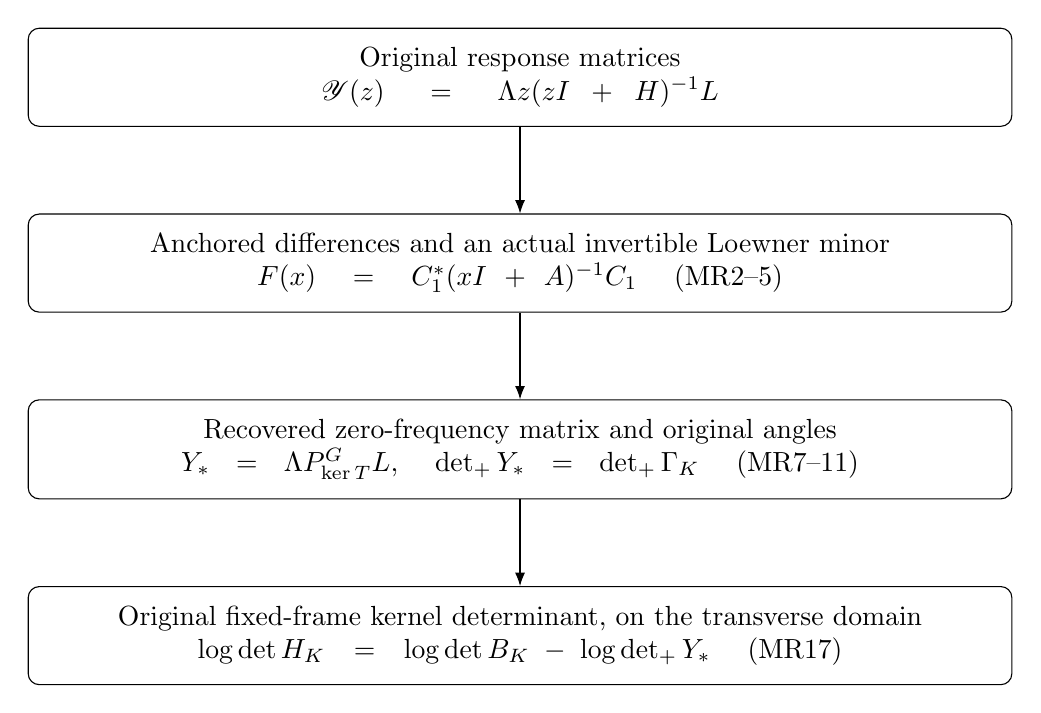
\begin{tikzpicture}[>=Latex,node distance=11mm,
 box/.style={draw,rounded corners,align=center,text width=12cm,inner sep=7pt}]
\node[box] (data) {Original response matrices\\
 $\mathscr Y(z)=\Lambda z(zI+H)^{-1}L$};
\node[box,below=of data] (rec) {Anchored differences and an actual invertible Loewner minor\\
 $F(x)=C_1^*(xI+A)^{-1}C_1$ \quad (MR2--5)};
\node[box,below=of rec] (end) {Recovered zero-frequency matrix and original angles\\
 $Y_*=\Lambda P_{\ker T}^G L$, \quad
 $\det_+Y_*=\det_+\Gamma_K$ \quad (MR7--11)};
\node[box,below=of end] (orig) {Original fixed-frame kernel determinant, on the transverse domain\\
 $\log\det H_K=\log\det B_K-\log\det_+Y_*$ \quad (MR17)};
\draw[->] (data)--(rec);\draw[->](rec)--(end);\draw[->](end)--(orig);
\end{tikzpicture}
\caption{Every arrow is a proved map in the original metric. The classical
Loewner factorization is credited to Mayo--Antoulas and to
Zhang--Gosea--Antoulas at the exact source locations in the proof.
Zero-angle intersections are retained in MR11 and SD10.
The scalar alternative uses $24k-64$ determinant samples at each cutoff,
with its sharp finite loss in SD6--7.}
\end{figure}
\[
0\le\mathcal K_k-\mathcal R[-\log\det_+Y_{*,N}]
\le2m\omega_k=o(kq),\qquad
\mathcal Rf=f_{q-1}+f_q-f_{2q-1}-f_{2q}.
\]
\clearpage
\section*{The polynomial quotient retains the current correction}
\addcontentsline{toc}{section}{The polynomial quotient retains the current correction}
The exact finite example in BD18 has two observation chains of lengths
$(2,1)$. Its original action and metric are printed in full there.
\[
 P(z)=\begin{pmatrix}z^2&z&1&0&0\\0&0&0&z&1\end{pmatrix},
\quad
 D(z)=\begin{pmatrix}1-z-z^3&-z^2\\-z&1-iz-z^2\end{pmatrix}.
\]
\begin{figure}[H]\centering
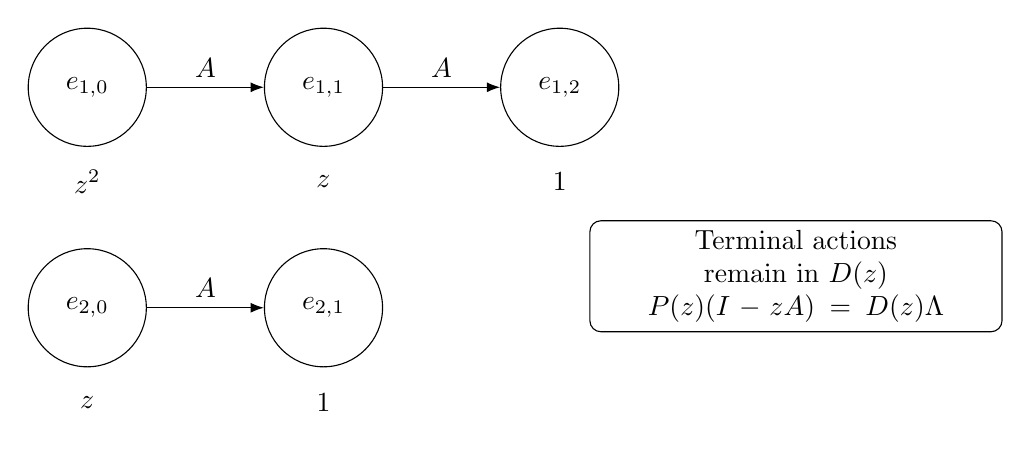
\begin{tikzpicture}[>=Latex]
\node[draw,circle,minimum size=15mm] (k10) at(0,1.8){$e_{1,0}$};
\node[draw,circle,minimum size=15mm] (k11) at(3,1.8){$e_{1,1}$};
\node[draw,circle,minimum size=15mm] (k12) at(6,1.8){$e_{1,2}$};
\draw[->](k10)--node[above]{$A$}(k11);
\draw[->](k11)--node[above]{$A$}(k12);
\node at(0,.6){$z^2$};\node at(3,.6){$z$};\node at(6,.6){$1$};
\node[draw,circle,minimum size=15mm](s0) at(0,-1){$e_{2,0}$};
\node[draw,circle,minimum size=15mm](s1) at(3,-1){$e_{2,1}$};
\draw[->](s0)--node[above]{$A$}(s1);
\node at(0,-2.2){$z$};\node at(3,-2.2){$1$};
\node[draw,rounded corners,align=center,text width=5cm] at(9,-.6)
 {Terminal actions remain in $D(z)$\\
 $P(z)(I-zA)=D(z)\Lambda$};
\end{tikzpicture}
\caption{The displayed arrows are the nonterminal action only.
They do not claim invariant cyclic summands.
The omitted terminal arrows are retained exactly by $D(z)$ (BD4--5).
The printed powers are the corresponding quotient-row coefficients.
The full coefficient Gram recovers the original source metric (BD9).}
\end{figure}
In this same example, for $b=(1,i)^{\mathsf T}$ and its original
attained output metric $Q$,
\[
 M_B=\mathcal C_{10}Q-D'(0),\qquad
 i b^*(QM_B-M_B^*Q)b=-\frac7{18}.
\]
Using only $\mathcal C_{10}Q$ gives $5/18$ instead.
The missing contribution is exactly $-2/3$.
These are auxiliary exact matrix values, not a native xi-packet sign.
\clearpage

\clearpage\part{Matrix recovery and every original angle}
\section{Finite matrix recovery and the original zero-frequency angle spectrum}\label{finite-matrix-recovery-and-the-original-zero-frequency-angle-spectrum}

This proof starts with the complete original observation and metric. The incoming anchored construction is proved in MR1--8. MR9--13 identify its recovered zero-frequency matrix directly with every primary angle, including intersections, zero directions and unit directions. MR14--17 give finite error and original determinant receivers. Finite recoverability does not assign the unevaluated original period values.

The predecessor is \href{https://github.com/KokunoYumeto/zeta-function-research-reader/blob/13ca9b136fcdae48df7454bd9bf99e1ef22dd03c/workbenches/splitzero-tandem/continuations/20260922-original-growth-resolvent/ORIGINAL_RESOLVENT_MEMORY_PROOFS.md}{RM1--23, exact kernel memory}. Its Schur construction is related to the Feshbach--Schur map of Geneviève Dusson, Israel Michael Sigal and Benjamin Stamm, \href{https://arxiv.org/abs/2105.02058v1}{arXiv:2105.02058v1}, Theorem1.2. The data factorization below is the Loewner realization method of A. J. Mayo and A. C. Antoulas, \href{https://doi.org/10.1016/j.laa.2007.03.008}{2007, DOI10.1016/j.laa.2007.03.008}, in the factorized form proved by Qiang Zhang, Ion Victor Gosea and Athanasios C. Antoulas, \href{https://arxiv.org/abs/2103.09674v1}{arXiv:2103.09674v1, Lemma2.1}. The latter original TeX, lines169--328, was read. Mayo--Antoulas is historical attribution; no original-TeX reading of that article is asserted. The finite original-metric proof is complete below.

\subsection{MR1. Original spaces, sections and energy}\label{mr1.-original-spaces-sections-and-energy}

Let \(E=\mathbb C^q\), \(G=G^*>0\), and let the fixed observation \(\Lambda:E\to B=\mathbb C^n\) be onto. Set \(K=\ker\Lambda\), \(m=q-n\), and retain its full column frame \(I_K:\mathbb C^m\to E\). Define \[
 Q=(\Lambda G^{-1}\Lambda^*)^{-1},\quad
 L=G^{-1}\Lambda^*Q,\quad H_K=I_K^*GI_K,\quad
 J_K=I_KH_K^{-1/2}.
\tag{MR1}
\] Then \(\Lambda L=I\), \(L^*GL=Q\), \(L^*GJ_K=0\), and \(J_K^*GJ_K=I_m\), by multiplication. Thus \(U=[L,J_K]\) is an invertible map from \(B\oplus\mathbb C^m\), carrying the metric \(\operatorname{diag}(Q,I)\) exactly to \(G\). These formulas preserve both original metrics rather than assigning Euclidean lengths to \(B\).

For the fixed word \(T:E\to E\), let \(H=G^{-1}T^*GT\), \(V=\ker T\), \(d=\dim V\), and \(\Delta=q-d\). Initially suppose \(K\cap V=0\); MR11 includes intersections. Choose a physical energy scale \(R\ge\|H\|_G>0\), and put \[
 A=R^{-1}J_K^*T^*GTJ_K,\quad
 C=R^{-1}J_K^*T^*GTL,\quad
 B_0=R^{-1}L^*T^*GTL.
\tag{MR2}
\] The matrix \(A\) is positive definite: its quadratic form is \(R^{-1}\|TJ_Kx\|_G^2\), and its kernel is the stated intersection. The whole energy form in \(U\) is \(\left(\begin{smallmatrix}B_0&C^*\\ C&A\end{smallmatrix}\right)\). Write \(\mathscr Y(z)=\Lambda z(zI+H)^{-1}L\).

\subsection{MR2. The anchored original measured response}\label{mr2.-the-anchored-original-measured-response}

Block elimination in \(U\), keeping the metric in MR1, gives for \(x>0\) \[
 \mathscr Y(Rx)=x[xQ+B_0-C^*(xI+A)^{-1}C]^{-1}Q.
\tag{MR3}
\] Indeed the top-left block of \((xU^*GU+U^*GHU/R)^{-1}\) is the displayed Schur inverse; multiplication by \(xQ\) on the right produces MR3. Define, in the original observation coordinates, \[
 Z(x)=xQ(\mathscr Y(Rx)^{-1}-I)
     =B_0-C^*(xI+A)^{-1}C.
\tag{MR4}
\] Subtract at \(x=1\), using the resolvent identity, and set \[
 C_1=(I+A)^{-1/2}C,\qquad
 F(x)=\frac{Z(x)-Z(1)}{x-1}
     =C_1^*(xI+A)^{-1}C_1 .
\tag{MR5}
\] The formula at1 is its derivative value, but the sampling scheme never asks for it.

Let \(\mathcal M=\operatorname{span}\{A^jCb:0\le j<m,b\in B\}\), \(s=\dim\mathcal M\). By Cayley--Hamilton this space is \(A\)-invariant, hence reducing because \(A=A^*\). Functional calculus and invertibility of \((I+A)^{1/2}\) on each eigenspace prove that \(C_1\) generates exactly the same space.

\subsection{MR3. Complete finite rank, including repeated poles}\label{mr3.-complete-finite-rank-including-repeated-poles}

When \(m>0\), use \(m\) nodes \(x_i=2+(i-1)/m\), and \(m\) nodes \(y_j=4+(j-1)/m\), together with the anchor1. Let \[
 \mathcal L_{ij}=\frac{F(x_i)-F(y_j)}{y_j-x_i},\qquad
 \mathcal S_{ij}=\frac{y_jF(y_j)-x_iF(x_i)}{y_j-x_i}.
\tag{MR6}
\] With \(X=[(A+x_iI)^{-1}C_1]_i\) and \(Y=[(A+y_jI)^{-1}C_1]_j\), direct subtraction gives \(\mathcal L=X^*Y\), \(\mathcal S=X^*AY\).

Both \(X\) and \(Y\) have range \(\mathcal M\). For proof, put \(p(t)=\prod_i(t+x_i)\). The polynomials \(p(t)/(t+x_i)\) form a basis of polynomials of degree at most \(m-1\): evaluation at \(-x_j\) proves independence. Multiplication by \(p(A)^{-1}\), invertible on the whole kernel, carries their span applied to \(C_1\) onto \(\mathcal M\). This is exactly the range of \(X\). The proof for \(Y\) is identical. It never requires distinct eigenvalues of \(A\).

Since \(X^*:\mathcal M\to B^m\) is injective and \(Y:B^m\to\mathcal M\) is onto, \(\operatorname{rank}\mathcal L=s\). This proves the actual memory rank from the finite data.

\subsection{MR4. Recovery through an actual nonzero minor}\label{mr4.-recovery-through-an-actual-nonzero-minor}

Choose row and column indices \(I,J\) giving an invertible \(s\)-square minor \(\mathcal L_0\), and take the same minor \(\mathcal S_0\). Let \(X_0,Y_0:\mathbb C^s\to\mathcal M\) be the selected columns of \(X,Y\). They are invertible onto \(\mathcal M\), since \(X_0^*Y_0=\mathcal L_0\). Set \[
 B_L=[F(x_i)]_{\text{selected rows}},\qquad
 B_R=[F(y_j)]_{\text{selected columns}}.
\] Then \(B_L=X_0^*C_1\), \(B_R=C_1^*Y_0\), and \[
 F(z)=B_R(\mathcal S_0+z\mathcal L_0)^{-1}B_L,\quad
 \mathcal L_0^{-1}\mathcal S_0=Y_0^{-1}A_{\mathcal M}Y_0 .
\tag{MR7}
\] Cancel the invertible factors \(X_0^*,Y_0\) to verify both equalities. The metric of the latter representation is \(Y_0^*Y_0\), which is retained; the matrix is not assigned Euclidean selfadjointness. For \(s=0\), \(C=0\), \(F=0\), and all subsequent empty determinants are1. The case \(m=0\) requires only \(Z(1)\).

Thus \(2m+1\) original matrix values suffice. This is a count of matrices, with exact entries; neither a bit-complexity estimate nor a value of the native period is implied.

\subsection{MR5. Two recovered zero coefficients}\label{mr5.-two-recovered-zero-coefficients}

Differentiate MR7 algebraically: \[
 F_0=B_R\mathcal S_0^{-1}B_L,\qquad
 F'_0=-B_R\mathcal S_0^{-1}\mathcal L_0\mathcal S_0^{-1}B_L.
\] The recovered forms are \[
 E_0=Z(1)-F_0=B_0-C^*A^{-1}C,\qquad
 W_0=F_0-F'_0=C^*A^{-2}C.
\tag{MR8}
\] To check the second equality on an eigenvalue \(a>0\), use \((a^{-1}+a^{-2})/(1+a)=a^{-2}\). For the first, use \(1/(1+a)+1/(a(1+a))=1/a\). The form \(E_0\) is the complete Schur minimum of the original energy and is positive semidefinite. The form \(W_0\) is the mass of the actual kernel graph; it has rank at most \(s\).

\subsection{MR6. Original zero space and its metric}\label{mr6.-original-zero-space-and-its-metric}

The zero space in \(U\) consists exactly of \[
 U\binom{b}{-A^{-1}Cb},\qquad b\in\ker E_0.
\tag{MR9}
\] This follows by completing the whole energy square: \[
 b^*E_0b+(a+A^{-1}Cb)^*A(a+A^{-1}Cb).
\] If \(Z_0\) is any full frame for \(\ker E_0\), the actual Gram of this graph is \[
 H_V=Z_0^*(Q+W_0)Z_0 .
\tag{MR10}
\] In particular \(\dim\ker E_0=d\). No coordinate volume in \(Z_0\) has been discarded.

\subsection{MR7. The zero-frequency matrix itself is recovered}\label{mr7.-the-zero-frequency-matrix-itself-is-recovered}

The spectral theorem in the \(G\) metric gives \[
 Y_*=\lim_{z\downarrow0}\mathscr Y(z)=\Lambda P_V^G L .
\tag{MR11}
\] Projection onto the graph MR9, using MR10, gives the explicit finite reconstruction \[
 \boxed{Y_*=Z_0[Z_0^*(Q+W_0)Z_0]^{-1}Z_0^*Q.}
\tag{MR12}
\] Indeed the graph frame is \(V_0=U[Z_0;-A^{-1}CZ_0]\); its observation is \(Z_0\), its adjoint against \(GL\) is \(Z_0^*Q\), and \(P_V^G=V_0(V_0^*GV_0)^{-1}V_0^*G\). If \(d=0\), the frame is empty and \(Y_*=0\). All matrices in MR12 are constructed from MR4--8 and the original \(Q\).

\subsection{MR8. Invisible memory and full original volume}\label{mr8.-invisible-memory-and-full-original-volume}

For \(w\in\mathcal M^\perp\), \(C^*w=0\), and \(A\) preserves \(\mathcal M^\perp\). Hence the subspace \(J_K\mathcal M^\perp\) is reducing for \(H\). It is positive and perpendicular to \(V\). Its primary-angle matrix is the identity. Its original kernel-coordinate Gram need not be the identity: \(J_K=I_KH_K^{-1/2}\) is the specified metric isometry, not a change to the fixed volume frame. Thus invisible memory cancels only unit angle factors; MR17 below retains \(H_K\).

\subsection{MR9. Full spectral morphism at zero frequency}\label{mr9.-full-spectral-morphism-at-zero-frequency}

This argument no longer requires \(K\cap V=0\). Define the primary matrix \[
 \Gamma_K=J_K^*GP_{V^{\perp_G}}^GJ_K,\qquad
 J_B=LQ^{-1/2},\qquad
 \overline Y_*=Q^{1/2}Y_*Q^{-1/2}=J_B^*GP_V^GJ_B .
\tag{MR13}
\] Both \(J_B,J_K\) are isometries, and their images are orthogonal complements in \(E\). Let \(J_V\) be a \(G\)-isometry from \(\mathbb C^d\) onto \(V\), and write \(A_V=J_K^*GJ_V\), \(B_V=J_B^*GJ_V\). Orthogonal resolution gives \(A_V^*A_V+B_V^*B_V=I_d\), while \(\Gamma_K=I_m-A_VA_V^*\) and \(\overline Y_*=B_VB_V^*\). Sylvester's determinant identity, itself obtained by eliminating the two blocks of \(\left(\begin{smallmatrix}I&X\\Y&I\end{smallmatrix}\right)\), yields the polynomial identity \[
 \boxed{(1-u)^m\det(I_n-u\overline Y_*)
       =(1-u)^d\det(I_m-u\Gamma_K).}
\tag{MR14}
\] For \(u\ne1\), replace \(B_V^*B_V\) by \(I_d-A_V^*A_V\) and apply that identity; multiplying clears every negative exponent. Polynomial equality then holds also at1. All eigenvalues in \((0,1)\) agree with complete multiplicities.

Here is the exact eigenvector map. For \(\Gamma_Kx=\gamma x\), \(0<\gamma<1\), put \(a=J_Kx\) and \[
 b=P_{K^{\perp_G}}^G P_V^G a,\qquad
 \Psi_\gamma x=\frac{J_B^*Gb}{\sqrt{\gamma(1-\gamma)}}.
\tag{MR15}
\] Since \(P_KP_Va=(1-\gamma)a\) and \(P_V^2=P_V\), one has \(P_BP_Vb=\gamma b\) and \(\|b\|_G^2=\gamma(1-\gamma)\|x\|^2\). Therefore \(\Psi_\gamma\) is an isometry onto the \(\gamma\) eigenspace of \(\overline Y_*\); the reverse construction or the equal multiplicity in MR14 proves surjectivity. This supplies the actual map, including complex phases.

\subsection{MR10. Zero, unit and positive determinants}\label{mr10.-zero-unit-and-positive-determinants}

Put \(t=\dim(K\cap V)\), \(a=\dim(K\cap V^{\perp_G})\), and \(b=\dim(K^{\perp_G}\cap V)\). Directly from the quadratic projection forms: \[
 \operatorname{null}\Gamma_K=t,\quad
 \operatorname{mult}_1\Gamma_K=a,\quad
 \operatorname{rank}Y_*=d-t,\quad
 \operatorname{mult}_1Y_*=b.
\tag{MR16}
\] The rank statement follows because \(P_B|_V\) has kernel \(K\cap V\); the compression is its product with its adjoint. The common count of eigenvalues strictly between0 and1 is \(h=m-t-a=d-t-b\), so \(b-a=d-m\). Consequently \[
 \boxed{\det\nolimits_+\Gamma_K=\det\nolimits_+Y_* .}
\tag{MR17}
\] The positive determinant is the product of positive eigenvalues; its empty value is1. Zero-angle multiplicity is not hidden in this convention: it is exactly \(t\) and must be reported with it. In the original transverse programme \(t=0\), so the left side is the ordinary primary determinant.

\subsection{MR11. Intersections in finite recovery}\label{mr11.-intersections-in-finite-recovery}

Let \(K_0=K\cap V\). In the metric coordinates MR1, \(A\) is positive semidefinite and its zero space corresponds exactly to \(K_0\). Positivity of the whole energy forces \(C^*|_{\ker A}=0\): the quadratic polynomial in a scalar multiple of a zero vector has nonnegative values for every complex scalar only if its linear cross coefficient vanishes. Thus the memory is entirely in \((\ker A)^\perp\). Restrict there, with \(p=m-t\), and replace \(A^{-1}\) by the positive-range inverse \(A^+\).

MR2--8 remain valid with at most \(2p+1\) samples if \(p\) is known; the \(2m+1\) scheme still works without reducing the count. The recovered graph is \(V\ominus_G K_0\); the missing zero space \(K_0\) is perpendicular to \(L(B)\), hence contributes zero to \(Y_*\). MR12 therefore still recovers exactly the same \(Y_*\), and MR16--17 include all original zero angles.

\subsection{MR12. Quantitative spectral approach to the recovered endpoint}\label{mr12.-quantitative-spectral-approach-to-the-recovered-endpoint}

Retain any proved positive spectral interval \(\ell P_{V^\perp}\preceq_G H\preceq_G uP_{V^\perp}\). For \(z>0\), put \(\tau_a=z/(z+a)\). Spectral calculus, followed by the actual isometry \(J_B\), proves \[
 \boxed{\overline Y_*+\tau_u(I-\overline Y_*)
 \preceq Q^{1/2}\mathscr Y(z)Q^{-1/2}
 \preceq\overline Y_*+\tau_\ell(I-\overline Y_*).}
\tag{MR18}
\] Let \(\beta_i(z)\) and \(y_i\) denote the decreasing ordered eigenvalues of the middle matrix and \(\overline Y_*\). Min--max gives the explicit enclosure \[
 \max\left(0,\frac{\beta_i(z)-\tau_\ell}{1-\tau_\ell}\right)
 \le y_i\le
 \min\left(1,\frac{\beta_i(z)-\tau_u}{1-\tau_u}\right).
\tag{MR19}
\] There is no assertion that coarse moderate-frequency data resolve arbitrarily small \(y_i\). Formula MR19 measures exactly how the gap and the actual response enter that question.

\subsection{MR13. A finite positive-determinant certificate}\label{mr13.-a-finite-positive-determinant-certificate}

Suppose a Hermitian approximation \(\widehat Y_*\) to \(\overline Y_*\) has operator error at most \(e\). Its known positive rank is \(r=d-t\). If the \(r\)-th decreasing eigenvalue \(\widehat y_r>e\), min--max gives \[
 -\sum_{i=1}^r\log\min(1,\widehat y_i+e)
 \le-\log\det\nolimits_+\Gamma_K
 \le-\sum_{i=1}^r\log(\widehat y_i-e).
\tag{MR20}
\] Only the known positive indices enter. Every logarithm has a strictly positive argument under the displayed guard. This certificate is for independent endpoint error; complete-source bounds in MR16 have a different, stronger error structure.

\subsection{MR14. Independent rounding in the anchored reconstruction}\label{mr14.-independent-rounding-in-the-anchored-reconstruction}

Use one fixed \(Q\)-isometry for error measurement. In those coordinates \(Q=I\) as a proved congruence, and \(x/(x+1)I\preceq\mathscr Y(Rx)\preceq I\). Suppose every original sample has error \(\eta\le1/4\), and all nonlinear operations below use the stated error intervals. Since \(\|Y^{-1}\|\le2\), the resolvent inverse identity gives error at most \(8\eta\) in each inverse. Therefore \(\|\delta Z(1)\|\le8\eta\), and on \(2\le x\le5\), \[
 \|\delta F(x)\|\le 8\eta(x+1)/(x-1)\le24\eta.
\] Every chosen scalar \(s\)-square minor consequently has \[
 e_L=48s\eta,\quad e_S=192s\eta,\quad
 e_{B_L}=e_{B_R}=24\sqrt s\,\eta.
\tag{MR21}
\] The separation \(y_j-x_i>1\) proves the first two bounds by entrywise estimates followed by Frobenius norm. The last two follow by stacking selected rows or columns.

Take actual upper bounds \(v\ge\|\mathcal S_0^{-1}\|\), \(l\ge\|\mathcal L_0\|\), \(b_L\ge\|B_L\|\), \(b_R\ge\|B_R\|\). Under \(ve_S<1\), set \(v'=v/(1-ve_S)\) and \[
 e_0=(b_R+e_{B_R})v'(b_L+e_{B_L})-b_Rvb_L,
\] \[
 e_1=(b_R+e_{B_R})(v')^2(l+e_L)(b_L+e_{B_L})
       -b_Rv^2lb_L.
\tag{MR22}
\] Expanding the product differences and using \(\|\delta(\mathcal S_0^{-1})\|\le v'-v\) proves \(\|\delta F_0\|\le e_0\), \(\|\delta F'_0\|\le e_1\). Hence \(e_E=8\eta+e_0\), \(e_W=e_0+e_1\) bound MR8. Taking Hermitian parts does not increase these errors.

\subsection{MR15. The energy gap gives the required kernel projector guard}\label{mr15.-the-energy-gap-gives-the-required-kernel-projector-guard}

In \(Q\)-isometric coordinates, the Schur form \(E_0\) is bounded by \[
 (\ell/R)P_{(K+V)^\perp}\preceq E_0
 \preceq (u/R)P_{(K+V)^\perp}.
\tag{MR23}
\] Here the projector is expressed in \(K^\perp\) via \(J_B\). To prove this, the Schur form of a vector \(b\) is the minimum of \(\langle H(b+a),b+a\rangle_G/R\) over \(a\in K\). Replace \(H\) by its lower or upper multiple of \(P_{V^\perp}\). The remaining minimum is \(\operatorname{dist}_G(b,K+V)^2\), proving MR23. Thus every positive eigenvalue of \(E_0\) is at least \(g_0=\ell/R\), without an extra angle factor.

Hermitian \(\widehat E_0\) with \(e_E<g_0/2\) has exactly the known number of zero-cluster eigenvalues in \([-e_E,e_E]\); the others are at least \(g_0-e_E\). Let \(\widehat P_0\) be the projector onto this cluster and \(P_0=\operatorname{proj}\ker E_0\). Then \(\|\widehat P_0-P_0\|\le2e_E/g_0\). For completeness, the off-diagonal block between \(\ker E_0\) and the complementary \(\widehat E_0\)-space solves a Sylvester equation whose spectra are separated by \(g_0-e_E\). Its inverse has norm at most \(1/(g_0-e_E)\), by the integral \(\int_0^\infty e^{-t\widehat E_{\rm high}}(\cdot)\,dt\). Multiplication by the perturbation gives the bound \(e_E/(g_0-e_E)\le2e_E/g_0\). Equal ranks identify this norm with the projector difference.

If \(M_W\ge\|W_0\|\), then \[
 e_{\rm ang}=e_W+4M_We_E/g_0
\tag{MR24}
\] bounds the difference between \(I+P_0W_0P_0\) and its hatted counterpart. The true determinant is \((\det_+\Gamma_K)^{-1}\): restrict to \(\ker E_0\) in MR10--12, or use Sylvester's identity. The true matrix is at least \(I\). Before taking Hermitian parts the reconstructed \(W_0\) has rank at most \(s\), afterward at most \(2s\); the difference of the two projected products has rank at most \(3s\). Thus, under \(e_{\rm ang}<1\), \[
 |\widehat{\mathcal J}-(-\log\det\nolimits_+\Gamma_K)|
 \le-\min(n,3s)\log(1-e_{\rm ang}).
\tag{MR25}
\] Indeed relative congruence by the true inverse square root puts every eigenvalue in \([1-e_{\rm ang},1+e_{\rm ang}]\), with at most \(\min(n,3s)\) eigenvalues different from1. Summing their logarithms proves the claim.

\subsection{MR16. Complete-source error has a rank cost}\label{mr16.-complete-source-error-has-a-rank-cost}

For fixed \(T,\Lambda,I_K\) and \(\alpha G\preceq\widetilde G\preceq\beta G\), let \(\kappa=\beta/\alpha\). The numerator form of every primary angle is \(\inf_{v\in V}\|I_Kx-v\|_G^2\); its denominator is \(\|I_Kx\|_G^2\). Both have the same complete-source enclosure. On the fixed quotient by \(K\cap V\), min--max gives \[
 \kappa^{-1}\gamma_j(G)\le\gamma_j(\widetilde G)\le\kappa\gamma_j(G).
\tag{MR26}
\] Consequently the positive determinant logarithms differ by at most \((m-t)\log\kappa\). Both minimum sections and both projections are recomputed from their actual metrics. This estimate is not a statement about independent sample perturbations.

\subsection{MR17. Return to the original four determinants}\label{mr17.-return-to-the-original-four-determinants}

On the transverse programme stratum \(T=D_k(M)\), the original primary quotient \(\pi_\partial\) has kernel \(V\). Its attained metric and restriction are \[
 G_N^\partial=(\pi_\partial G_N^{-1}\pi_\partial^*)^{-1},\qquad
 B_{K,N}=(\pi_\partial I_K)^*G_N^\partial(\pi_\partial I_K).
\] By the quotient minimum, \(B_{K,N}=I_K^*G_NP_{V^{\perp_{G_N}}}I_K\). Therefore MR17 proves the absolute identity \[
 \boxed{\log\det H_{K,N}
 =\log\det B_{K,N}-\log\det\nolimits_+Y_{*,N}.}
\tag{MR27}
\] All constant coordinate determinants stay in both sides. Write \(\mathcal R f_N=f_{q-1}+f_q-f_{2q-1}-f_{2q}\) and \(\mathcal J_N=-\log\det_+Y_{*,N}\). The retained boundary-width result \href{https://github.com/KokunoYumeto/zeta-function-research-reader/blob/9b7b0bad40b33dc88bba7d8cb1548da1fadbb585/workbenches/splitzero-tandem/continuations/20260921-original-angle-word/ANGLE_PROOFS.md}{AS, original angle proof} supplies \(a_kI\preceq G_N^\partial\preceq b_kI\), \(\omega_k=\log(b_k/a_k)=O(k\log q)\), with decreasing cutoff metrics. Hence \[
 \boxed{0\le\mathcal K_k-\mathcal R\mathcal J_N
 \le2m\omega_k=o(kq).}
\tag{MR28}
\] Proof: congruence by the same \(\pi_\partial I_K\) preserves the finite width; decreasing metrics make each low-minus-high log determinant nonnegative, and each is at most \(m\omega_k\). There are two such pairs.

Combining MR28 with the exact \href{https://github.com/KokunoYumeto/zeta-function-research-reader/blob/13ca9b136fcdae48df7454bd9bf99e1ef22dd03c/workbenches/splitzero-tandem/continuations/20260922-original-growth-resolvent/GROWTH_PROOFS.md}{RG50--54 finite invariant receiver}, whose finite bound is \(|\mathcal K_k-\log\mathcal A_k+G_0+G_1|\le\mathcal E_k\), gives \[
 -\mathcal E_k\le
 \log\mathcal A_k-G_0-G_1-\mathcal R\mathcal J_N
 \le\mathcal E_k+2m\omega_k.
\tag{MR29}
\] Thus the scalar invariant-row return and the full matrix endpoint are joined by a proved directed bound, without identifying their differently ranked angle matrices.

\subsection{MR18. Exact complex replay}\label{mr18.-exact-complex-replay}

Take \(G=I_4\), \(\Lambda=(I_2,0)\), \[
 T=\begin{pmatrix}1&i&1&0\\0&1/\sqrt2&0&\sqrt2\\0&0&0&0\\0&0&0&0\end{pmatrix}.
\] Its positive energies are2 and7/2; \(R=4\) is allowed. Put \(C_*=\left(\begin{smallmatrix}1&i\\0&1\end{smallmatrix}\right)\). The three original samples at \(x=1,2,4\) give \[
 F(2)=C_*^*\operatorname{diag}(1/45,1/60)C_*,
 \quad F(4)=C_*^*\operatorname{diag}(1/85,1/108)C_*.
\] Here one block minor already has full memory rank2, so three samples suffice. They yield \[
 \mathcal L_0=C_*^*\operatorname{diag}(4/765,1/270)C_*,
 \quad\mathcal S_0=C_*^*\operatorname{diag}(1/765,1/540)C_*,
\] \[
 E_0=0,\quad W_0=C_*^*\operatorname{diag}(1,1/4)C_*,
 \quad Y_*=(I+W_0)^{-1}
 =\begin{pmatrix}9/14&-2i/7\\2i/7&4/7\end{pmatrix}.
\] Direct projection gives \(\Gamma_K=\left(\begin{smallmatrix}5/14&-i/7\\i/7&6/7\end{smallmatrix}\right)\). They are different coordinate matrices, related by MR15; both have determinant \(2/7\) and eigenvalues \((17\pm\sqrt{65})/28\). This tests the full complex reconstruction and spectral morphism. It is an auxiliary exact example, not evaluated original xi data.

\subsection{MR19. Precision is an actual mathematical datum}\label{mr19.-precision-is-an-actual-mathematical-datum}

For fixed \(T=\operatorname{diag}(0,1)\), \(\Lambda=(-1,1)\), and \(G_\varepsilon=\operatorname{diag}((1-\varepsilon)/\varepsilon,1)\), direct inversion gives \(Q=1-\varepsilon\), \(\mathscr Y_\varepsilon(z)=(z+\varepsilon)/(z+1)\), \(Y_*=\Gamma_K=\varepsilon\), and \(H_K=1/\varepsilon\). If \(\varepsilon=2^{-L}\) and \(\varepsilon'=2^{-L-q}\), then on \([1,5]\) the response difference is at most \(2^{-L-1}\), whereas the primary determinant logarithms differ by \(q\log2\). Direct sums multiply this logarithmic difference by the kernel rank. The exact endpoint and finite recovery formulas retain that information, but recovering it from independently rounded samples requires corresponding precision. None of MR1--29 replaces it by a rank count.

\clearpage\part{Scalar recovery and its sharp information loss}
\section{Scalar recovery, every primary angle, and the complete complementary energy minimum}\label{scalar-recovery-every-primary-angle-and-the-complete-complementary-energy-minimum}

Independent derivation, 22 September 2026. The complete supplied 04\_received.md was read; 05\_received.md is its identical copy. The original source and observation definitions of 01\_received.md and 03\_received.md are retained. Every statement below is finite unless its asymptotic specialization is explicitly identified. The actual period-dependent scalar samples and the residual \(kq\) coefficient remain unevaluated.

The supplied transverse scalar interpolation and logarithmic-angle bounds are valid. Their complete rank-changing extension uses \(p=\operatorname{rank}(TI_K)\), not the full kernel dimension in the positive list. Beyond those statements, the scalar leading coefficient and the complete complementary energy minimum give a sharper determinant interval of optimal dimension-dependent width. This continuation derives that interval, its exact connecting map and its original-kernel receiver.

\subsection{SD1. Original metric, maps, and all ranks}\label{sd1.-original-metric-maps-and-all-ranks}

Let \(E=\mathbb C^q\) have the original positive Hermitian metric \(G\), let the full original observation \(\Lambda:E\to B\) be onto, and put \[
\begin{gathered}
K=\ker\Lambda,\quad m=\dim K,\quad b=\dim B=q-m,\\
Q=(\Lambda G^{-1}\Lambda^*)^{-1},\quad
L=G^{-1}\Lambda^*Q,\quad H_K=I_K^*GI_K.
\end{gathered}
\tag{SD1}
\] Here \(I_K:\mathbb C^m\hookrightarrow E\) is the fixed full original kernel frame. Direct multiplication gives \(\Lambda L=I\), \(L^*GL=Q\), and \(I_K^*GL=0\). Thus \([L,J_K]\), where \(J_K=I_KH_K^{-1/2}\), gives an orthogonal decomposition with metric \(\operatorname{diag}(Q,I_m)\).

Retain the actual word \(T\) and define \[
\begin{gathered}
H=G^{-1}T^*GT,\quad V=\ker T=\ker H,\quad
\Delta=\operatorname{rank}T,\quad d=q-\Delta,\\
K_0=K\cap V,\quad t=\dim K_0,\quad p=m-t,\quad \delta_+=\Delta-p.
\end{gathered}
\tag{SD2}
\] All these ranks are algebraic; no numerical threshold defines them. Positivity gives \(\ker(J_K^*GHJ_K)=J_K^{-1}K_0\), so \(p=\operatorname{rank}(TI_K)\le\Delta\) and \(\delta_+\ge0\). Let \[
A_K=J_K^*GHJ_K,\qquad
\Gamma=J_K^*GP_{V^{\perp_G}}J_K,\qquad
\mathscr Y(z)=\Lambda z(zI+H)^{-1}L,\qquad f(z)=\det_B\mathscr Y(z).
\tag{SD3}
\] Both \(A_K\) and \(\Gamma\) have the same kernel \(J_K^{-1}K_0\). On its Euclidean orthogonal complement, equivalently the attained metric quotient \(K/K_0\), write their positive restrictions as \(A_+\) and \(\Gamma_+\). Their \(p\) eigenvalues are positive; \(0<\Gamma_+\preceq I_p\). Empty determinants are one.

For the original simple-quartet family, \[
k\equiv1\pmod4,\quad k\ge17,\quad q=(k+1)^2,\quad
m=8k-16,\quad\Delta=16k-48,\quad d=(k-7)^2.
\tag{SD4}
\] The real roots remain \(\omega_{ab}=(2b-k)\gamma-i(2a-k)\delta\), \(0<\delta<1/2\), \(\gamma>2\). The coefficient action is \(M[p]=[yp]\) on \(\mathbb C[y]/Q_k\), the physical action is \(kI/2+iM\), and \(T=D_k(M)\) uses the full original pivot-translated interior word. The original conductor proves \(K\cap V=0\), so here \(t=0,p=m,\delta_+=8k-32\). The full \(\Lambda\), all invariant constraints, the original physical unit, and each arithmetic metric \(G_N\) remain unchanged.

The coefficient transport \(S\) acts simultaneously by \(T'=STS^{-1}\), \(G'=S^{-*}GS^{-1}\), \(\Lambda'=\Lambda S^{-1}\), \(L'=SL\), \(H'=SHS^{-1}\); hence \(\mathscr Y'=\mathscr Y\) exactly. A common source mass \(aG\) changes \(Q,H_K\) by \(a\) and leaves \(L,H,\mathscr Y,A_K,\Gamma\) unchanged. This verifies metric balancing without discarding an actual source mass.

\subsection{SD2. Complete scalar determinant and multiplicities}\label{sd2.-complete-scalar-determinant-and-multiplicities}

In the frame \([L,J_K]\), put \(B_E=L^*GHL\), \(C=J_K^*GHL\). The form of \(zI+H\) is \[
\begin{pmatrix}zQ+B_E&C^*\\ C&zI_m+A_K\end{pmatrix}.
\] For \(z>0\), elimination of the full lower block gives \[
\mathscr Y(z)=z\,[zQ+B_E-C^*(zI_m+A_K)^{-1}C]^{-1}Q.
\] Its determinant, including the metric determinant \(Q\), is therefore \[
f(z)=z^{q-m}\frac{\det(zI_m+A_K)}{\det(zI_q+H)}
=z^{\delta_+}
\frac{\prod_{j=1}^{p}(z+\alpha_j)}
{\prod_{j=1}^{\Delta}(z+\lambda_j)}.
\tag{SD5}
\] Here every positive eigenvalue \(\alpha_j\) of \(A_K\) and \(\lambda_j\) of \(H\) is listed with full multiplicity. Indeed the numerator before positive-factor extraction has \(t\) zero factors and the denominator has \(d\), so its zero order is \(q-m+t-d=\Delta-p\). The determinant calculation uses \(\det(zI+H)=\det(\text{displayed form})/\det Q\); this is why no \(Q\)-factor is missing.

This is also the rank-changing formula PR7--8 in the \href{https://github.com/KokunoYumeto/zeta-function-research-reader/blob/13ca9b136fcdae48df7454bd9bf99e1ef22dd03c/workbenches/splitzero-tandem/continuations/20260922-original-growth-resolvent/RECEIVED_RESOLVENT_PROOFS.md}{original measured-resolvent proof}, rederived here directly from the original forms. The Feshbach--Schur construction is treated by Geneviève Dusson, Israel Michael Sigal and Benjamin Stamm, Theorem 1.2 and equations labelled Fesh and QP in their \href{https://arxiv.org/abs/2105.02058}{original author source, arXiv:2105.02058}. The finite determinant and rank accounting in (SD5) are proved above.

For each \(a>0\), define its two multiplicities \(n_A(a)\), \(n_H(a)\). The common divisor has multiplicity \(\min(n_A(a),n_H(a))\); the reduced numerator and denominator retain respectively \[
n_{\rm num}(a)=(n_A(a)-n_H(a))_+,\qquad
n_{\rm den}(a)=(n_H(a)-n_A(a))_+.
\tag{SD6}
\] This definition permits repeated energies and exact cancellations without identifying cancellation with matrix-memory invisibility.

Fix a proved positive spectral interval \[
\ell P_{V^{\perp_G}}\preceq_G H\preceq_G uP_{V^{\perp_G}},
\qquad0<\ell\le u,\qquad w=\log(u/\ell).
\tag{SD7}
\] If \(\Delta=0\), \(H=0\), \(p=0\), and \(f=1\); no positive spectral interval is needed. When \(\Delta>0\), every \(0<\alpha<\ell\) has \(n_H(\alpha)=0\), and therefore survives with its entire multiplicity. Equality \(\alpha=\ell\) is deliberately excluded from that conclusion.

The full zero multiplicity of \(\Gamma\) is exactly \(t\). Among its \(p\) positive eigenvalues, at most \[
a_{\max}=\min(p,d-t)
\tag{SD8}
\] are nonunit. To prove this, \(I-\Gamma_+\) is the Gram of the map from \(K_0^{\perp_G}\cap K\) to \(V\). Its image is perpendicular to \(K_0\), because the original vector is perpendicular to \(K_0\subset V\). Thus its rank is at most \(\dim(V\cap K_0^{\perp_G})=d-t\), and also at most \(p\). This bound retains unit factors even when \(d<m\).

\subsection{SD3. Every logarithmic angle and inverse exterior rank}\label{sd3.-every-logarithmic-angle-and-inverse-exterior-rank}

Congruence of (SD7) by \(J_K\), then restriction to the positive part, gives \[
\ell\Gamma_+\preceq A_+\preceq u\Gamma_+.
\tag{SD9}
\] Order both positive eigenvalue lists increasingly. Rayleigh min--max gives \(\ell\gamma_j\le\alpha_j\le u\gamma_j\) in that same ordering. This needs no commutation. Put \(h_j=-\log\gamma_j\), so \(h_1\ge\cdots\ge h_p\ge0\).

The reduced scalar numerator determines exactly \[
\widehat h_j=(\log(\ell/\alpha_j))_+,\qquad1\le j\le p,
\tag{SD10}
\] by taking every subgap factor, retaining its multiplicity, and padding the decreasing list with zeros to length \(p\). A missing canceled positive energy is at least \(\ell\), so contributes exactly zero to this list.

If \(\alpha_j\le\ell\), then \(h_j-\widehat h_j=\log(\alpha_j/(\ell\gamma_j))\in[0,w]\). If \(\alpha_j>\ell\), then \(\gamma_j\ge\alpha_j/u>\ell/u\), so \(0\le h_j<w\) and \(\widehat h_j=0\). Hence \[
0\le h_j-\widehat h_j\le w,\qquad
h_j=\widehat h_j=0\quad(j>a_{\max}),
\tag{SD11}
\] and for all \(0\le r\le p\), \[
0\le\sum_{j=1}^r(h_j-\widehat h_j)\le\min(r,a_{\max})w.
\tag{SD12}
\] This includes every positive exterior rank and improves the rank coefficient when the zero-word space is smaller.

The actual map is \[
J=P_{V^{\perp_G}}J_{K,+}:\mathbb C^p\longrightarrow V^{\perp_G}.
\] Its image has the inherited original \(G\)-metric; \(J^*GJ=\Gamma_+\). Thus its inverse on that actual image has squared singular values \(1/\gamma_1,\ldots,1/\gamma_p\). Therefore \[
e^{\sum_{j=1}^r\widehat h_j}
\le\|\wedge^r(J^{-1}|_{\operatorname{im}J})\|^2
\le e^{\min(r,a_{\max})w+\sum_{j=1}^r\widehat h_j}.
\tag{SD13}
\] If \(t>0\), the unreduced map on all \(K\) is not injective. Its \(t\) zero singular values are retained; an inverse on all \(K\) is not asserted. Equation (SD13) refers to its exact attained quotient, or equivalently the inverse into \(K_0^{\perp_G}\cap K\).

For every \(s\ge0\), \[
\#\{j:h_j>s+w\}\le\#\{j:\widehat h_j>s\}
\le\#\{j:h_j>s\}.
\tag{SD14}
\] After division by a common \(q\), the ordered lists differ in \(W_\infty\) by at most \(w/q\), and in every \(W_r\), \(1\le r<\infty\), by at most the same amount. Any common centering leaves this statement unchanged. For \(p=0\) use the empty list, not an undefined empirical probability measure.

\subsection{SD4. The entire retained numerator sharpens the ordered upper bound}\label{sd4.-the-entire-retained-numerator-sharpens-the-ordered-upper-bound}

Let \(\mathscr A_{\rm ret}\) be all reduced numerator energies in physical units, with cardinality \(n\), and let \(c=p-n\) be the cancellation degree. Form an increasing list \[
a_1^-\le\cdots\le a_p^-
\quad\text{from }\mathscr A_{\rm ret}\cup\{\ell\}^{c}.
\tag{SD15}
\] The actual positive energy list is obtained by replacing these \(c\) copies of \(\ell\) by the actual canceled energies, each at least \(\ell\). Therefore \(a_j^-\le\alpha_j\) at every index. All energies are at most \(u\), because \(A_+\preceq u\Gamma_+\preceq uI\). Define \[
\beta_j=\begin{cases}\log(u/a_j^-),&j\le a_{\max},\\0,&j>a_{\max}.\end{cases}
\tag{SD16}
\] This is decreasing and nonnegative. Min--max and (SD8) give the complete ordered enclosure \[
\widehat h_j\le h_j\le\beta_j,\qquad
0\le\beta_j-\widehat h_j\le w.
\tag{SD17}
\] For the second inequality before the forced-zero tail, use \(\widehat h_j=(\log(\ell/a_j^-))_+\). If \(a_j^-\le\ell\), the interval width is \(w\); if \(a_j^->\ell\), it is \(\log(u/a_j^-)\le w\). This also proves that the forced-zero tail of the lower list really is zero.

Put \[
U=\sum_{j=1}^{p}\widehat h_j,\qquad V_{\rm ret}=\sum_{j=1}^{p}\beta_j.
\tag{SD18}
\] Then \(U\le-\log\det\Gamma_+\le V_{\rm ret}\), with \(V_{\rm ret}-U\le a_{\max}w\). Without the rank improvement \(a_{\max}\), the upper endpoint is exactly \(\sum_{\alpha\in\mathscr A_{\rm ret}}\log(u/\alpha)+c\,w\), the supplied equation (10). For every exterior rank one may instead sum the first \(r\) terms in (SD17). The midpoint list \(b_j=(\widehat h_j+\beta_j)/2\) is ordered, satisfies \[
|h_j-b_j|\le(\beta_j-\widehat h_j)/2\le w/2,
\tag{SD19}
\] and hence approximates each logarithmic angle with half the maximum interval width. This is a two-sided estimate; it does not claim a stronger one-sided error for the original lower list.

\subsection{SD5. Exact scalar interpolation, including all cancellations}\label{sd5.-exact-scalar-interpolation-including-all-cancellations}

Choose \(R\ge\|H\|_G\), with \(R>0\). Define \(\mathcal L=p+\Delta\). If \(\mathcal L=0\), \(f=1\) and zero samples suffice. Otherwise use the distinct nodes \[
x_i=1+i/\mathcal L,\quad z_i=Rx_i,\quad0\le i<\mathcal L,
\quad r_i=x_i^{-\delta_+}f(Rx_i).
\tag{SD20}
\] All lie in \([R,2R)\). The underlying rational function is \[
r_R(x)=x^{-\delta_+}f(Rx)
=\frac{P(x)}{D(x)},\quad
P(x)=\prod_{j=1}^p(x+\alpha_j/R),\quad
D(x)=\prod_{j=1}^{\Delta}(x+\lambda_j/R).
\tag{SD21}
\] The powers of \(R\) cancel because \(\delta_+=\Delta-p\); the roots still carry their exact physical scale.

Both polynomials are monic. Their lower coefficients solve \[
\sum_{j<p}a_jx_i^j-r_i\sum_{j<\Delta}b_jx_i^j
=r_ix_i^\Delta-x_i^p,\quad0\le i<\mathcal L.
\tag{SD22}
\] For any solution \(P_1,D_1\), compare with the actual \(P,D\). The polynomial \(P_1D-PD_1\) vanishes at all nodes and has degree at most \(p+\Delta-1=\mathcal L-1\), since the leading terms cancel. It is identically zero. Thus every solution represents the same rational function after exact common-factor cancellation. A solution may have both numerator and denominator zero at a sample node; cancel their gcd before evaluation. Such an intermediate \(0/0\) does not invalidate the polynomial proof.

More precisely, let \(P_0,D_0\) be the coprime monic reduced pair, of degrees \(n=p-c\), \(d_0=\Delta-c\). Coprimality and \(P_1D_0=P_0D_1\) imply \[
P_1=P_0S,\qquad D_1=D_0S,
\quad S\text{ arbitrary monic of degree }c.
\tag{SD23}
\] For example \(P_0\mid P_1\) follows by Bézout: multiply \(UP_0+VD_0=1\) by \(P_1\) and use the cross-product equality. Monicity fixes \(S\)'s leading coefficient. Conversely every such \(S\) solves (SD22). Therefore the interpolation system has nullity exactly \(c\), including repeated common factors. If the reduced degrees have been established separately, \(n+d_0=p+\Delta-2c\) distinct samples suffice by the same argument. No distinct-energy or generic-rank assumption was used.

In the native transverse family, \(\mathcal L=\Delta+m=24k-64\). Rank-changing data use the actual \(\Delta+p\), with the zero order \(\Delta-p\); the unreduced full formula (SD5) remains valid at every rank transition.

For the sample bound, \(z(zI+H)^{-1}\) lies between \(x/(x+1)\) and \(1\) when \(z=Rx\), \(x\ge1\). Compress by the original minimum-section isometry. Moreover the difference from identity has rank at most \(\min(b,\Delta)\). Hence \[
\left({x\over x+1}\right)^{\min(b,\Delta)}
\le f(Rx)\le1.
\tag{SD24}
\] In particular \(2^{-\Delta}\le f(Rx)\le1\) on the stated interval. This controls measured positive matrices and scalar values; it does not bound interpolation conditioning or the number of bits required for tiny positive roots.

\subsection{SD6. The scalar leading coefficient and complete complementary energy minimum}\label{sd6.-the-scalar-leading-coefficient-and-complete-complementary-energy-minimum}

The scalar data determine \[
a_{\rm sc}=\lim_{z\downarrow0}z^{-\delta_+}f(z)
=\frac{\det A_+}{\det(H|_{V^{\perp_G}})}
=R^{-\delta_+}\frac{P_0(0)}{D_0(0)}>0.
\tag{SD25}
\] The limit is calculated by the recovered polynomial constants, with no further response samples or limiting numerical operation.

Let \(F=P_{V^{\perp_G}}J_{K,+}\), so \(F^*GF=\Gamma_+\), and put \(U_K=F\Gamma_+^{-1/2}\). This is an isometry onto \(P_{V^{\perp_G}}K\). Complete it by a \(G\)-isometry \(Z\) onto its orthogonal complement in \(V^{\perp_G}\), of dimension \(\delta_+\). In this exact orthonormal frame the positive energy is \[
\begin{pmatrix}\mathcal A&\mathcal C\\
\mathcal C^*&\mathcal D\end{pmatrix},\qquad
\Sigma=\mathcal D-\mathcal C^*\mathcal A^{-1}\mathcal C.
\] The image lies in \(V^{\perp_G}\), and \(H\) annihilates \(V\), so \(A_+=\Gamma_+^{1/2}\mathcal A\Gamma_+^{1/2}\). Block elimination then proves \[
a_{\rm sc}=\frac{\det\Gamma_+}{\det\Sigma},
\qquad
\det\Gamma_+=a_{\rm sc}\det\Sigma,
\qquad
\Sigma^{-1}=Z^*G(H|_{V^{\perp_G}})^{-1}Z.
\tag{SD26}
\] The off-diagonal energy block is retained. The transverse identity is precisely PR8a in the cited original measured-resolvent proof; the present proof extends it to the actual quotient at \(t>0\).

The meaning of \(\Sigma\) is the attained energy on each fixed complementary fibre: \[
y^*\Sigma y=\min_{x\in\mathbb C^p}
\left\langle U_Kx+Zy,H(U_Kx+Zy)\right\rangle_G.
\] Since the frame is orthonormal, (SD7) implies \[
\ell I_{\delta_+}\preceq\Sigma\preceq uI_{\delta_+}.
\tag{SD27}
\] For the lower bound minimize \(\ell(\|x\|^2+\|y\|^2)\); for the upper bound choose \(x=0\). Consequently, with \(S_{\rm sc}=-\log a_{\rm sc}\), \[
S_{\rm sc}-\delta_+\log u
\le-\log\det\Gamma_+
\le S_{\rm sc}-\delta_+\log\ell.
\tag{SD28}
\] No individual scalar numerator root is needed for this interval.

Intersect the two independently proved intervals: \[
L_{\rm sc}=\max\{U,S_{\rm sc}-\delta_+\log u\},\qquad
U_{\rm sc}=\min\{V_{\rm ret},S_{\rm sc}-\delta_+\log\ell\}.
\tag{SD29}
\] They contain the actual determinant, so \(L_{\rm sc}\le U_{\rm sc}\), and \[
0\le U_{\rm sc}-L_{\rm sc}
\le \min(p,d-t,\Delta-p)\,\log(u/\ell).
\tag{SD30}
\] Thus the best certified scalar ambiguity here is governed by the positive kernel dimension, the available zero-word dimension, and the complementary positive-energy dimension. For \(\Delta=p\), (SD26) has an empty complementary determinant and scalar leading-coefficient recovery of \(\det\Gamma_+\) is exact even for a nonflat positive spectrum. Flat spectra also give exact recovery of every positive angle, by (SD9).

\subsection{SD7. Sharp examples in every admissible dimension}\label{sd7.-sharp-examples-in-every-admissible-dimension}

For \(u>\ell>0\), take \(G=I_3\), \(\Lambda(x_1,x_2,x_3)=(x_1,x_2)\), \(K=\mathbb Ce_3\), and \[
H_0=\operatorname{diag}(u,0,\ell),\qquad
H_1=\begin{pmatrix}
u-\ell&0&\sqrt{\ell(u-\ell)}\\
0&\ell&0\\
\sqrt{\ell(u-\ell)}&0&\ell
\end{pmatrix}.
\tag{SD31}
\] They are \(T_i^*T_i\) for \(T_0=\operatorname{diag}(\sqrt u,0,\sqrt\ell)\) and \[
T_1=\begin{pmatrix}\sqrt{u-\ell}&0&\sqrt\ell\\
0&\sqrt\ell&0\\0&0&0\end{pmatrix}.
\] Both have full energies \(\{0,\ell,u\}\), \(A_K=\ell\), \(Q=I_2\), and \[
\mathscr Y_0(z)=\operatorname{diag}(z/(z+u),1),\quad
\mathscr Y_1(z)=\operatorname{diag}((z+\ell)/(z+u),z/(z+\ell)).
\tag{SD32}
\] Hence both determinants equal \(z/(z+u)\), while \(\Gamma_0=1,\Gamma_1=\ell/u\). The second system's kernel coupling is nonzero. Its scalar cancellation of \(z+\ell\) is not a reducing invisible direction of matrix memory. The two \(\Sigma\) values are respectively \(u,\ell\), realizing both endpoints of (SD28).

For arbitrary admissible \(q,m,\Delta,t\), set \[
s_*=\min(p,\Delta-p,d-t).
\tag{SD33}
\] Take \(s_*\) copies of (SD31); add \(p-s_*\) positive kernel-only modes, \(\Delta-p-s_*\) positive observed-only modes, \(t\) zero kernel-only modes, and \(d-t-s_*\) zero observed-only modes. Every count is nonnegative. The total dimension is \(3s_*+(p-s_*)+(\Delta-p-s_*)+t+(d-t-s_*)=q\); the kernel dimension is \(p+t=m\), the positive-word rank is \(\Delta\), and its intersection rank is \(t\). All added blocks agree between the two systems. Thus their scalar data, full positive spectra, observed metrics and algebraic ranks agree, but \[
\left|\log\det\Gamma_{+,1}-\log\det\Gamma_{+,0}\right|
=s_*\log(u/\ell).
\tag{SD34}
\] This proves sharpness of the dimension-dependent ambiguity coefficient in (SD30), even with the full positive spectrum supplied in addition to all scalar response values. On the auxiliary pair, each nonunit logarithmic-angle error also attains \(w\); direct sums attain (SD12) wherever the indicated nonunit ranks are available. These examples are finite positive-word systems; they are not asserted to be native xi-packet data.

\subsection{SD8. A finite scalar surrogate without individual root extraction}\label{sd8.-a-finite-scalar-surrogate-without-individual-root-extraction}

In addition to the leading coefficient, the reconstructed rational function itself gives an explicit approximation to the subgap statistic \(U\). Let \(n=\deg P_0\), \(d_0=\deg D_0\), and \(\tau=\ell/R>0\). Put \[
\Psi=\log\frac{r_R(\tau)}{r_R(0)}
=\log\frac{P_0(\tau)D_0(0)}{D_0(\tau)P_0(0)}.
\tag{SD35}
\] All arguments of logarithms are positive. This uses evaluations of the recovered polynomials; it does not request another original response sample.

For each retained numerator energy, \[
0\le\log(1+\ell/\alpha)-(\log(\ell/\alpha))_+\le\log2.
\] For each retained denominator energy, \(\lambda\ge\ell\), so \(0\le\log(1+\ell/\lambda)\le\log2\). Expanding (SD35) over their full multiplicities proves \[
-n\log2\le U-\Psi\le d_0\log2.
\tag{SD36}
\] Thus a ratio of four recovered polynomial values approximates the whole subgap sum within a degree-dependent finite error, even when some numerator roots are arbitrarily small or repeated. In the original family \(n,d_0=O(k)\), this added error is \(O(k)\). It does not assert that computing a very small positive polynomial value requires few bits.

There is also an exact root-independent integral map. In physical units let \(r(z)=z^{-\delta_+}f(z)\). For \(0<a<\ell\) avoiding numerator roots on the circle, factor its polynomials and use the mean-value identity for each \(z+\alpha\). This gives \[
\frac1{2\pi}\int_0^{2\pi}
\log\left|\frac{r(ae^{i\theta})}{r(0)}\right|\,d\theta
=\sum_{\alpha<a}\log(a/\alpha).
\tag{SD37}
\] Denominator factors give zero because their roots lie outside the circle. At boundary zeros, their logarithmic singularities are integrable: for one factor the identity follows directly from the power-series mean outside its root radius and from factoring the radius inside; continuity in the radius follows by integrating \(\log|e^{i\theta}-r|\), or by its explicit value \(\log^+r\). Letting \(a\uparrow\ell\) proves that the same integral at the endpoint, interpreted by this integrable limit, equals \(U\). This connects the exact multiplicity-counted clipping to the recovered scalar holomorphic function without declaring any quadrature error negligible.

\subsection{SD9. Original arithmetic receiver and its complete finite spectral width}\label{sd9.-original-arithmetic-receiver-and-its-complete-finite-spectral-width}

At the four original cutoffs \(N\in\{q-1,q,2q-1,2q\}\), use \(\mathcal RF=f_{q-1}+f_q-f_{2q-1}-f_{2q}\). The original boundary map has kernel \(V\), and \[
G_N^\partial=(\pi_\partial G_N^{-1}\pi_\partial^*)^{-1},\qquad
\widehat H_{K,N}^\partial=(\pi_\partial I_K)^*G_N^\partial(\pi_\partial I_K).
\] The exact minimum over the original affine fibres gives \[
\Gamma_N=H_{K,N}^{-1/2}\widehat H_{K,N}^\partial H_{K,N}^{-1/2},
\quad
\log\det H_{K,N}=\log\det\widehat H_{K,N}^\partial-\log\det\Gamma_N.
\tag{SD38}
\] Indeed the \(G_N\)-minimum lift of each boundary value is its projection to \(V^{\perp_{G_N}}\); its squared norm is the boundary quotient norm. This proves (SD38) with the actual minimum, without replacing it by a coefficient metric.

The original word provider gives a common boundary comparison \(a_kI\preceq G_N^\partial\preceq b_kI\) and source nesting \(G_{N+1}^\partial\preceq G_N^\partial\). Since \(\pi_\partial I_K\) is fixed and injective, each low-to-high log-determinant drop lies in \([0,m\log(b_k/a_k)]\). Thus \[
0\le\mathcal R\log\det\widehat H_{K,N}^\partial
\le B_\partial:=2m\omega_k,\qquad\omega_k=\log(b_k/a_k).
\tag{SD39}
\] All constants here retain their original arithmetic source. Explicitly, writing \(R_h=\sqrt{\delta^2+\gamma^2}\) and \(R_k=kR_h\), \[
a_k=\ell_k/A_{2q}^\partial,\quad b_k=u_kB_k^\partial,\quad
A_{2q}^\partial=\frac{\Delta e^2}{M_\sigma}(2q+1)^{3/2}(4q+1)^{R_k+1},
\] \[
B_k^\partial=\Delta M_\sigma
\left(\frac{2\Delta+R_k}{2\delta}\right)^{2(\Delta-1)},\qquad M_\sigma=\sqrt{2\pi}.
\] Here \(\ell_k,u_k\) are the original full-mass arithmetic/Gamma comparison constants of the word provider, not the positive energy thresholds \(\ell_N,u_N\).

For precision at the \(kq\) scale, retain the complete original image-Gram enclosure \(e^{c_N-\epsilon_k}I\preceq\mathfrak G_N\preceq e^{c_N+\epsilon_k}I\). Its parameter and equilibrium status are those of the proved/imported original word source, not newly inferred from scalar interpolation. The exact original image map is \(J=V_O^{-1}\pi_\partial I_K\), and \(H_{TK,N}=J^*\mathfrak G_NJ\). The full Vandermonde and Lagrange constants are \[
V_+=\Delta\max(1,R_k)^{\Delta-1},\qquad
V_-=\Delta\left(\frac{1+R_k}{2\delta}\right)^{\Delta-1},
\] \[
E_k=\epsilon_k+
\max\{\log^+(b_kV_+^2),\log^+(V_-^2/a_k)\}.
\tag{SD40}
\] The positive word operator is exactly \((G_N^\partial)^{-1/2}V_O^{-*}\mathfrak G_NV_O^{-1}(G_N^\partial)^{-1/2}\). Taking both norm bounds and inverse norm bounds proves \[
e^{c_N-E_k}\le\lambda_{j,N}^+\le e^{c_N+E_k}.
\tag{SD41}
\] These are \href{https://github.com/KokunoYumeto/zeta-function-research-reader/blob/13ca9b136fcdae48df7454bd9bf99e1ef22dd03c/workbenches/splitzero-tandem/continuations/20260922-original-growth-resolvent/RECEIVED_RESOLVENT_PROOFS.md}{PR19--22 of the pinned original measured-resolvent proof}. Its retained original domain gives \(E_k=o(q)\), \(\omega_k=O_{h,\varpi}(k\log q)=o(q)\), and \[
c_{\rm L}=2q\log q+(2\log(4/\pi)-2)q,\qquad
c_{\rm H}=c_{\rm L}-C_\partial q/2.
\tag{SD42}
\] The low type is \(q-1,q\), the high type is \(2q-1,2q\). The finite scalar theorems SD1--37 themselves require only the measured maps and a finite positive spectral interval; no unproved value of \(C_\partial\) enters them.

Set \(\ell_N=e^{c_N-E_k},u_N=e^{c_N+E_k}\). The supplied angle comparison follows: \(0\le h_{j,N}-\widehat h_{j,N}\le2E_k=o(q)\). The original four-sign receiver is \[
\mathcal R U_N-2E_k(a_{\max,2q-1}+a_{\max,2q})
\le\mathcal K_k
\le\mathcal R U_N+2E_k(a_{\max,q-1}+a_{\max,q})+B_\partial.
\tag{SD43}
\] On the transverse native family \(a_{\max,N}=\min(m,d)\), independent of \(N\); replacing it by \(m\) gives exactly the incoming \(4mE_k\) bounds. For separate finite widths \(w_N\), replace each \(2E_ka_{\max,N}\) by \(w_Na_{\max,N}\). This also explains every sign in the directed interval.

The leading coefficient yields a second receiver with no individual-root calculation: \[
\rho_N=\frac{P_{0,N}(0)}{D_{0,N}(0)},\qquad
\Theta_N=-\log\rho_N+\delta_+(\log R_N-c_N).
\tag{SD44}
\] A separate certified scale \(R_N\) is permitted and is explicitly retained. From (SD26),(SD41), \[
|-\log\det\Gamma_N-\Theta_N|\le\delta_+E_k,
\] and consequently \[
\mathcal R\Theta_N-4\delta_+E_k
\le\mathcal K_k
\le\mathcal R\Theta_N+4\delta_+E_k+B_\partial.
\tag{SD45}
\] When one common \(R\) is used, \(\mathcal Rc_N=C_\partial q\), so this is the explicit scalar-constant receiver \[
-4\delta_+E_k
\le
\mathcal K_k+\mathcal R\log\rho_N+\delta_+C_\partial q
\le4\delta_+E_k+B_\partial,
\quad\delta_+=8k-32.
\tag{SD46}
\] It determines the same residual \(kq\)-scale coefficient from the recovered scalar constants, up to the stated \(o(kq)\) remainder. No positive regularizer is taken numerically to zero.

For the sharpest finite determinant interval, use (SD29) at each cutoff: \[
L_{q-1}+L_q-U_{2q-1}-U_{2q}
\le\mathcal K_k
\le U_{q-1}+U_q-L_{2q-1}-L_{2q}+B_\partial.
\tag{SD47}
\] Here \(L_N=L_{{\rm sc},N}\), \(U_N=U_{{\rm sc},N}\) only in (SD47). With \(M_N=(L_N+U_N)/2\), it follows that \[
\left|\mathcal K_k-\mathcal RM_N-B_\partial/2\right|
\le\frac12\sum_N(U_N-L_N)+B_\partial/2.
\tag{SD48}
\] For the native data the sum is at most \(8s_*E_k\), where \(s_*=\min(m,\Delta-m,d)\). This centers a fully specified interval; it does not assume that the unknown boundary determinant equals its midpoint.

To connect with the actual lower-root invariant rows, retain \(g=\Delta-v\), their complete projected covariance gains \(G_0,G_1\), and the exact scalar \(\mathcal A_{k,v}\) from \href{https://github.com/KokunoYumeto/zeta-function-research-reader/blob/13ca9b136fcdae48df7454bd9bf99e1ef22dd03c/workbenches/splitzero-tandem/continuations/20260922-original-growth-resolvent/GROWTH_PROOFS.md}{RG50--54}. That finite theorem gives \(|\mathcal K_k-\log\mathcal A_{k,v}+G_0+G_1|\le\mathcal E_k\). Combining it with (SD45) yields \[
-\mathcal E_k-4\delta_+E_k
\le \log\mathcal A_{k,v}-G_0-G_1-\mathcal R\Theta_N
\le \mathcal E_k+4\delta_+E_k+B_\partial.
\tag{SD49}
\] Every root, original row and complementary minimum remains in those gains. This exact directed connection does not identify the rank-\(m\) primary-angle operator with the rank-\(r_k\) lower-root projection. Under the original outer receiver with its retained error \(E_{\rm out}\), \(|\mathcal K_k-gC_\partial q-\mathcal R\log\det S_N|\le E_{\rm out}\), substitution in (SD45) gives the same interval enlarged by \(E_{\rm out}\) for \(gC_\partial q+\mathcal R\log\det S_N-\mathcal R\Theta_N\). Thus the original scalar \(g\), full lower-root ideal and unresolved invariant-row coefficient are all preserved.

\subsection{SD10. Rank-changing kernel metrics and coherent source errors}\label{sd10.-rank-changing-kernel-metrics-and-coherent-source-errors}

At \(t>0\), the preceding scalar statements recover the positive determinant, not the zero factors' metric. Here is the exact missing factor in the original coordinates. Choose a fixed full frame \([I_0,I_1]=I_KS\) of \(K\), with \(I_0\) spanning \(K_0\), and write \[
S^*H_KS=\begin{pmatrix}H_{00}&H_{01}\\H_{01}^*&H_{11}\end{pmatrix},
\qquad H_{\rm quot}=H_{11}-H_{01}^*H_{00}^{-1}H_{01}.
\] Let \(B_{11}=I_1^*GP_{V^{\perp_G}}I_1\). The boundary form annihilates \(K_0\), so its matrix in this frame is \(\operatorname{diag}(0,B_{11})\). The nonzero generalized spectrum against \(S^*H_KS\) is that of \((B_{11},H_{\rm quot})\): block inversion gives its lower inverse block \(H_{\rm quot}^{-1}\). Therefore \[
\det_+\Gamma=\frac{\det B_{11}}{\det H_{\rm quot}},\qquad
\log\det H_K
=\log\det H_{00}+\log\det B_{11}
-\log\det_+\Gamma-2\log|\det S|.
\tag{SD50}
\] This is the complete connecting map at an intersection. The fixed \(S\)-factor cancels under four original signs; the original \(H_{00}\) factor does not disappear.

Its possible invisibility is exact, not a universal reconstruction claim: take \(T=\operatorname{diag}(0,1)\), \(\Lambda=(0,1)\), and \(G_a=\operatorname{diag}(a,1)\), \(a>0\). Then \(K_0=K=\mathbb Ce_1\), \(f(z)=z/(z+1)\) for every \(a\), but \(\det H_K=a\). The positive metric cone on \(K_0\) is the exact defect space in this example, and (SD50) states how it re-enters the full kernel determinant. For \(m=0\), all kernel determinants are empty and \(f(z)=z^\Delta/\prod(z+\lambda_j)\). For \(T=0\), \(p=\Delta=0\), \(f=1\), and \(\Gamma=0_m\); only the zero-dimensional positive quotient has determinant one. A logarithm of the full zero determinant is not replaced by zero.

Now suppose two complete original source forms satisfy \(aG\preceq\widetilde G\preceq bG\), \(0<a\le b\), \(\kappa=b/a\), with the same \(T,\Lambda,I_K\). Restriction to \(K\), restriction of the image form \(I_K^*T^*GTI_K\), and attained quotients by the fixed \(K_0\) retain these same two constants: minimize the corresponding inequalities on each identical affine fibre. Generalized min--max gives \[
\kappa^{-1}\alpha_j(G)\le\alpha_j(\widetilde G)\le\kappa\alpha_j(G),
\quad
\kappa^{-1}\gamma_j(G)\le\gamma_j(\widetilde G)\le\kappa\gamma_j(G).
\tag{SD51}
\] For the second statement use the complete boundary quotient by \(V\), then restrict it to \(K/K_0\); its numerator and denominator forms both retain factors \(a,b\). With one common valid threshold \(\ell\), logarithmic clipping is 1-Lipschitz, and both clipped lists have at most \(a_{\max}\) positive entries. Therefore \[
|U(\widetilde G)-U(G)|\le a_{\max}\log\kappa,\qquad
|\log\det_+\Gamma(\widetilde G)-\log\det_+\Gamma(G)|
\le a_{\max}\log\kappa.
\tag{SD52}
\] Every rank-\(r\) positive inverse exterior logarithm has error at most \(\min(r,a_{\max})\log\kappa\).

The leading coefficient also has an explicit coherent bound. The complementary space in SD6 is \((K+V)^{\perp_G}\). On the fixed quotient \(E/(K+V)\), minimize the energy \(x^*T^*GT x\) and the metric \(x^*Gx\) on the same affine fibres. The energy minimum is attained: after factoring out \(V\), its form is positive definite and the remaining minimization is an ordinary positive quadratic minimum. Its positive generalized matrix relative to the metric minimum is exactly \(\Sigma\). Both quotient forms inherit the factors \(a,b\), so \(|\log\det\Sigma(\widetilde G)-\log\det\Sigma(G)|\le\delta_+\log\kappa\). Together with (SD26),(SD52), \[
|\log a_{\rm sc}(\widetilde G)-\log a_{\rm sc}(G)|
\le(a_{\max}+\delta_+)\log\kappa.
\tag{SD53}
\] The sections, adjoints and minima must all be recomputed from their respective complete metrics. Independent rounding of scalar samples does not satisfy these hypotheses.

Indeed for the fixed \(T=\operatorname{diag}(0,1)\), \(\Lambda=(-1,1)\), and \(G_\varepsilon=\operatorname{diag}((1-\varepsilon)/\varepsilon,1)\), \[
f_\varepsilon(z)=\frac{z+\varepsilon}{z+1},\qquad
\Gamma_\varepsilon=\varepsilon,\qquad0<\varepsilon<1.
\tag{SD54}
\] For \(\varepsilon=2^{-L}\), \(\varepsilon'=2^{-L-q}\), the response difference on \([1,2]\) is at most \(2^{-L-1}\), while the angle logarithms differ by \(q\log2\). Every positive full-word energy equals one. Exact interpolation and sharp spectral-width bounds therefore do not remove the needed small-root or small-constant precision.

\subsection{SD11. Verification and provenance}\label{sd11.-verification-and-provenance}

The companion exact checker verifies the full physical determinant under nonunitary complex coordinate transport, common-factor multiplicities and interpolation nullities, kernel/word intersections, zero words and empty kernels, the complete complementary Schur identity, dimension-dependent sharp examples, coherent metric errors and finite polynomial-value receivers. Normal and optimized-mode receipts record the proof and checker hashes. These checks are finite auxiliary systems, not evaluations of native period-dependent matrices.

Original human-source reading is recorded precisely in \path{SOURCE_USE_LEDGER.md} and JSON. The author TeX of Dusson--Sigal--Stamm is used for the classical Feshbach--Schur context. The polynomial uniqueness argument SD20--23 is proved directly here, independently of a general Loewner realization theorem. Mayo--Antoulas (2007), retained from the incoming bibliography, is contextual attribution, not an assertion that its unavailable author source was read. Zhang, Gosea and Antoulas (2021), arXiv:2103.09674, supplies an accessible original-TeX primary treatment of the separate matrix Loewner factorization, with its actual reading extent recorded. Existing020 proofs and their human attributions are preserved.

\clearpage\part{Bounded arithmetic probes and complete source control}
\section{Finite observation chains with the original source and current}\label{finite-observation-chains-with-the-original-source-and-current}

Independent derivation, 22 September 2026. The received sources are \texttt{03\_received.md} and \texttt{06\_received.md}; both were read completely. Statements BD1--BD18 below prove the bounded-degree receiver and add an intrinsic degree theorem, an explicit whole-source metric estimate, and recovery of every original spectral-pole residue. The original native kernel coefficient and the separate complex-current signs remain unevaluated. No conclusion here supplies the inherited EIQ value.

\subsection{BD1. Original objects and the admitted period domain}\label{bd1.-original-objects-and-the-admitted-period-domain}

Fix the original simple hypothetical offcritical quartet, with \(0<\delta<1/2\), \(\gamma>2\), and the actual original unit and period. Retain the size-five orbit domain and the stronger period bound OC71--73, \(|\varpi|\ge R_{\rm corner}^{\rm explicit}\), which proves all four corner coefficients nonzero. Its proof uses \(\gamma\ge1000\delta\); for an actual zeta quartet this follows from the retained Platt--Trudgian finite-height theorem. These are existing proved programme domains, not new assumptions substituted for an unfinished calculation. The exact definitions and proof coverage are recorded in \texttt{\path{SOURCE_USE_LEDGER.md}}.

Let \(k\equiv1\pmod4\), \(k\ge17\), and put \[
q=(k+1)^2,\quad m=8k-16,\quad n=q-m,\quad
\omega_{ab}=(2b-k)\gamma-i(2a-k)\delta,
\] \[
Q_k(y)=\prod_{a,b=0}^k(y-\omega_{ab}),\qquad
E=\mathbb C[y]/(Q_k),\quad M[p]=[yp],\quad
\mathscr A=kI/2+iM.
\] All roots are distinct, since their real and imaginary parts recover \(b,a\). All roots are nonzero, since \(k\) is odd. The given observation \(\Lambda:E\to B\) is onto, \(\dim B=n\), and \(K=\ker\Lambda\) has dimension \(m\). For every original cutoff \(q-1\le N\le2q\), \(G_N>0\) is the actual attained metric obtained by minimizing the original polynomial-source norm on its entire affine fibre. No Euclidean metric replaces \(G_N\).

The original conductor biform has coefficients \(a_{uv}\), \(0\le u,v\le8\), including every original scalar and phase, and \[
\sigma_{uv}=(2v-8)\gamma-i(2u-8)\delta,
\quad C_A[p]=\left[\sum_{u,v=0}^8a_{uv}p(y+\sigma_{uv})\right]
\in E_-:=\mathbb C[y]/Q_{k-8}.
\] Original CP8--9 prove well-definedness and a unique onto map \(\widehat C_A:B\to E_-\) with \(C_A=\widehat C_A\Lambda\). Indeed \(S=k/2+iy\), \(S_-=(k-8)/2+iy_-\) transforms CP8's physical shift \(4+(2u-8)\delta+i(2v-8)\gamma\) into exactly the displayed \(\sigma_{uv}\). This is a coordinate identity, including the centering and \(i\), and does not move the physical integration axis.

The precise public proofs are \href{https://github.com/KokunoYumeto/zeta-function-research-reader/blob/13ca9b136fcdae48df7454bd9bf99e1ef22dd03c/workbenches/splitzero-tandem/continuations/20260922-original-growth-resolvent/RETAINED_COMPLETE_PROOF_SOURCES.tex\#L128308}{OC71--73, complete original corner bound} and \href{https://github.com/KokunoYumeto/zeta-function-research-reader/blob/13ca9b136fcdae48df7454bd9bf99e1ef22dd03c/workbenches/splitzero-tandem/continuations/20260922-original-growth-resolvent/RETAINED_COMPLETE_PROOF_SOURCES.tex\#L279817}{OC61, the finite-height domain}. Dave Platt and Tim Trudgian's \href{https://arxiv.org/abs/2004.09765}{original paper, arXiv:2004.09765}, Theorem 1 (source label bank), proves height \(3\,000\,175\,332\,800\); the weaker \(3\cdot10^{12}\) suffices here. Its retained original author TeX was read through the theorem and the complete ``Theory and computation'' section. This task does not rerun that finite-height computation.

The conductor maps and their proof are retained in \href{https://github.com/KokunoYumeto/zeta-function-research-reader/blob/13ca9b136fcdae48df7454bd9bf99e1ef22dd03c/workbenches/splitzero-tandem/continuations/20260922-original-growth-resolvent/RETAINED_COMPLETE_PROOF_SOURCES.tex\#L281873}{CP8--9, original conductor and arithmetic defect}. The matching source lines were inspected; an unrelated occurrence of the prefix IVO is not used as evidence for this map.

\subsection{BD2. Literal restriction maps and the 80-power bound}\label{bd2.-literal-restriction-maps-and-the-80-power-bound}

Use the root-value isomorphisms solely as coordinates. For \(s=(u,v)\), define \[
(R_sx)_{ab}=x_{a+u,b+v}\quad(0\le a,b\le k-8).
\] Then \(C_A=\sum_s a_sR_s\) and \(R_sM-M_-R_s=\sigma_sR_s\). The latter follows entry by entry from \(\omega_{a+u,b+v}^{(k)}-\omega_{ab}^{(k-8)}=\sigma_{uv}\). Induction gives \[
C_j:=\sum_s a_s\sigma_s^jR_s
=\sum_{h=0}^j(-1)^{j-h}\binom jh M_-^{j-h}C_AM^h. \tag{BD2}
\] Let \(\mathcal S=\{s:a_s\ne0\}\), \(J=|\mathcal S|\le81\). The shifts on this support are distinct. Write \[
L_s(z)=\prod_{t\in\mathcal S\setminus\{s\}}\frac{z-\sigma_t}{\sigma_s-\sigma_t}
=\sum_{j=0}^{J-1}\ell_{sj}z^j.
\] The identity \(\sum_j\ell_{sj}C_j=a_sR_s\) is exact. Thus the observations \(\Lambda M^h\), \(0\le h\le J-1\), recover every supported restriction \(R_s\), with the actual nonzero \(a_s\) divided only where allowed. Each corner box is a product of intervals \([0,k-8]\) or \([8,k]\). Their union covers \([0,k]^2\), since \(k\ge17\). Every upper coordinate is therefore recovered. Consequently \[
\bigcap_{h=0}^{J-1}\ker(\Lambda M^h)=0,\qquad d\le J-1\le80. \tag{BD3}
\] Without the corner domain, this argument recovers precisely the union of supported boxes for the conductor stack. It does not identify \(\Lambda\) with \(C_A\), nor prove a failure of the original observation from a failure of that smaller stack.

\subsection{BD3. Eight derivatives leave at most 128 directions}\label{bd3.-eight-derivatives-leave-at-most-128-directions}

Homogenize the actual conductor as a biform \(\mathcal A\) of bidegree \((8,8)\) in \((X_0,X_1;Y_0,Y_1)\), and put \[
\mathcal D=-2i\delta X_1\partial_{X_1}+2\gamma Y_1\partial_{Y_1}.
\] Its monomial weights are \(-2i\delta u+2\gamma v\), pairwise distinct within any bidegree. The constant difference between these weights and \(\sigma_{uv}\) means the spans of the first \(r+1\) derivative biforms and moment biforms coincide, by an invertible triangular binomial matrix.

No coordinate variable divides \(\mathcal A\), because its four corners are nonzero. If a nonconstant bihomogeneous irreducible \(f\mid\mathcal A\) satisfied \(f\mid\mathcal Df\), equal bidegrees would give \(\mathcal Df=cf\). Distinct weights force \(f\) to be one monomial. An irreducible monomial is a coordinate variable, a contradiction. Thus \(f\nmid\mathcal Df\).

If \(f\) has multiplicity \(e\) in \(\mathcal A\), then \(e\le8\): at least one positive coordinate of the bidegree of \(f\) uses at least \(e\) of the corresponding total degree eight. Leibniz's formula gives \[
\mathcal D^e(f^eg)\equiv e!(\mathcal Df)^eg\pmod f,\qquad f\nmid g,
\] because every other distribution of the \(e\) derivatives leaves an undifferentiated factor \(f\). Hence \(\gcd(\mathcal A,\mathcal D\mathcal A,\ldots,\mathcal D^8\mathcal A)=1\), with multiplicities treated explicitly.

There are at most sixteen distinct irreducible factors: their positive total bidegrees sum to sixteen counting multiplicity. For each factor \(f\), the polynomial \(\sum_{j=1}^8t^{j-1}\mathcal D^j\mathcal A\) modulo \(f\) is nonzero and has degree at most seven in \(t\). The quotient by the prime \(f\) is an integral domain, so it has at most seven scalar zeros. Among \(t=0,\ldots,112\), at least one therefore gives a biform \(\mathcal B\) coprime to \(\mathcal A\).

In the biform ring, multiplication by \(\mathcal A\) and \(\mathcal B\) on bidegree \((k-8,k-8)\) is injective. Their images intersect in \(\mathcal A\mathcal B\mathcal P_{k-16,k-16}\): unique factorization implies \(\mathcal A u=\mathcal Bv\) only when \(u=\mathcal Bw\), \(v=\mathcal Aw\). Thus the sum has codimension \[
(k+1)^2-2(k-7)^2+(k-15)^2=128. \tag{BD4}
\] The ordinary transposes of these multiplication matrices are precisely the root-coordinate convolution maps. Ordinary transpose determines their rank; no Hermitian source metric is inserted into this algebraic identification. Since \(C_A=\widehat C_A\Lambda\), (BD2) shows that \[
K_j:=\bigcap_{h=0}^j\ker(\Lambda M^h),\qquad \dim K_8\le128. \tag{BD5}
\] This proves the claimed constant for the original observation even though the conductor generally has a larger kernel. It uses no squarefreeness assertion.

\subsection{BD4. Partial chains, their construction, and their intrinsic lengths}\label{bd4.-partial-chains-their-construction-and-their-intrinsic-lengths}

Put \(R=k\sqrt{\delta^2+\gamma^2}\), \(\nu=2R\), and \(A=M/\nu\). This changes only the receiver parameter; the original operator remains \(M=\nu A\) and the source measure is unchanged. Let \(d\) be least with \(K_d=0\). Multiplication gives injective maps \[
A:K_j/K_{j+1}\longrightarrow K_{j-1}/K_j.
\] Indeed \(Ax\in K_{j-1}\) for \(x\in K_j\), and \(Ax\in K_j\) implies \(x\in K_{j+1}\). Define \(b_j=\dim K_{j-1}-\dim K_j\), \(1\le j\le d\), \(b_{d+1}=0\). These injections prove \(b_{j+1}\le b_j\).

For each \(j\), descending from \(d\) to one, choose a complement of \(K_j+AK_j\) in \(K_{j-1}\). Its dimension is \(b_j-b_{j+1}\): the image of \(AK_j\) in \(K_{j-1}/K_j\) has dimension \(b_{j+1}\). For each chosen vector \(x\), take \(x,Ax,\ldots,A^jx\). Inductively, at quotient level \(K_{r-1}/K_r\), the descendants of longer selected chains span the injected copy of \(K_r/K_{r+1}\), and the vectors newly selected at level \(r\) complete its basis. Descending induction proves all nonterminal vectors form a basis of \(K\). At level \(E/K\), the terminal vectors of positive-length chains are independent: a relation modulo \(K\) among their terminals would, after taking their immediate predecessors, contradict the injectivity \(K/K_1\to E/K\). Add terminal-only chains to complete \(E/K\).

We obtain a basis \(F\) with chains \[
e_{a,0},\ldots,e_{a,\varepsilon_a},\quad
Ae_{a,j}=e_{a,j+1}\ (j<\varepsilon_a),\quad a=1,\ldots,n.
\] The nonterminal vectors span \(K\). Terminal actions are unrestricted; they remain in \(\widehat A=F^{-1}AF\). With coordinate inclusions \(E_K,E_B\) for nonterminal and terminal vectors, respectively, \(\Lambda F=R_B E_B^*\) for an invertible \(R_B\). Precisely, \[
\dim K_j=\sum_a(\varepsilon_a-j)_+,\quad
\#\{a:\varepsilon_a\ge j\}=b_j,\quad
\sum_a\varepsilon_a=m,\quad \max_a\varepsilon_a=d\le80,
\] \[
\sum_a(\varepsilon_a-8)_+\le128,\quad
b_1\ge(m-128)/8=k-18,\quad
\sum_a\varepsilon_a^2\le8m+80\cdot128. \tag{BD6}
\] For the last bound, \(\varepsilon^2\le8\varepsilon+80(\varepsilon-8)_+\) when \(0\le\varepsilon\le80\). A negative lower bound for \(b_1\) is simply weaker than \(b_1\ge0\). These are partial observation chains, not invariant cyclic summands.

\subsection{BD5. The polynomial quotient and its complete finite spectral data}\label{bd5.-the-polynomial-quotient-and-its-complete-finite-spectral-data}

Define the \(n\times q\) matrix \(P(z)\) by a separate row on each chain, \[
P_a(z)=(z^{\varepsilon_a},z^{\varepsilon_a-1},\ldots,z,1).
\] Its supports are disjoint. Directly on each nonterminal column, \[
P(z)(I-z\widehat A)E_K=0,\quad P(z)E_B=I,\quad
D(z):=P(z)(I-z\widehat A)E_B,
\] \[
P(z)(I-z\widehat A)=D(z)E_B^*,\qquad D(0)=I. \tag{BD7}
\] The matrix \(U(z)=[(I-z\widehat A)E_K,E_B]\) is polynomial and unimodular. In each chain its columns are \(e_j-ze_{j+1}\) followed by the terminal \(e_\varepsilon\); their determinant is one in chain order. Reordering all hidden columns before all terminals contributes only a fixed sign. Its bottom inverse rows are \(P(z)\), since they annihilate the first columns and equal the identity on terminal columns. Consequently \[
U(z)^{-1}(I-z\widehat A)[E_K,E_B]
=\begin{pmatrix}I&X(z)\\0&D(z)\end{pmatrix}.
\] An upper block column operation removes \(X\). All transformations are unimodular; evaluating at zero fixes the scalar determinant. Therefore \[
\det D(z)=\det(I-zM/\nu),\qquad
\operatorname{coker}_{\mathbb C[z]}D\simeq
\operatorname{coker}_{\mathbb C[z]}(I-zM/\nu). \tag{BD8}
\] The forward map is \(PF^{-1}\); the inverse is terminal inclusion in the displayed transformed quotient. This proves equality of every finite elementary divisor, including its algebraic multiplicity, not only equality of determinants. The original \(M\) has no zero eigenvalue. For an unrelated operator with a zero eigenvalue, affine cokernels would not record that eigenvalue at infinity; (BD8) makes no such assertion.

\subsection{BD6. New intrinsic degree and minimality theorem}\label{bd6.-new-intrinsic-degree-and-minimality-theorem}

Every polynomial row \(T(z)\) satisfying \(T(z)(I-z\widehat A)E_K=0\) obeys \(Te_{a,j}=zTe_{a,j+1}\), one column at a time. It follows exactly that \[
T(z)=u(z)P(z),\qquad u(z)=T(z)E_B. \tag{BD9}
\] Thus the annihilator is a free polynomial module with basis the rows of \(P\). Since the supports of those rows are disjoint, no highest-degree cancellation between distinct chains is possible, and \[
\deg(uP)=\max_{a:u_a\ne0}(\deg u_a+\varepsilon_a).
\] The dimension of its rows of degree at most \(h\) is therefore \[
H(h)=\sum_a\max(h-\varepsilon_a+1,0). \tag{BD10}
\] The second finite differences of \(H\) give the number of chains of each length. Hence the multiset \(\{\varepsilon_a\}\) is intrinsic to the observation pair, and \(d\) is its necessary maximum polynomial basis degree. Any other polynomial module basis is \(VP\) with \(V\) unimodular; its row degrees cannot all be less than \(d\), because then those rows could not generate a chain coordinate with length \(d\). This proves degree minimality without assuming any cyclic invariance.

The number 80 is sharp for the conductor-support argument alone. For any distinct \(J\) shifts set \(a_s=1/\prod_{t\ne s}(\sigma_s-\sigma_t)\). Lagrange interpolation of \(z^j\) gives \(\sum_s a_s\sigma_s^j=0\) for \(0\le j<J-1\), and one for \(j=J-1\). All coefficients are nonzero. The constant upper value vector then vanishes under every conductor observation through power \(J-2\), by the binomial formula, but not at \(J-1\). Taking the full original \(9\times9\) shift rectangle gives \(J-1=80\). This is a sharpness example for arbitrary conductor coefficients with the stated support; it does not identify those coefficients with the actual period product or claim the actual full observation requires 80 powers.

\subsection{BD7. The projective quotient retains all endpoints}\label{bd7.-the-projective-quotient-retains-all-endpoints}

Homogenize the row on chain \(a\) to \((z^{\varepsilon_a},z^{\varepsilon_a-1}w,\ldots,w^{\varepsilon_a})\). Its kernel is spanned by \(we_j-ze_{j+1}\). At every projective point these vectors are independent: if \(w\ne0\), solve sequentially from the first coordinate; if \(w=0\), they are nonzero multiples of distinct \(e_{j+1}\). Their number is the kernel dimension. Thus the complete exact sequence is \[
0\longrightarrow\mathcal O(-1)^m\longrightarrow\mathcal O^q
\longrightarrow\bigoplus_a\mathcal O(\varepsilon_a)\longrightarrow0. \tag{BD11}
\] At \(z=0\) the terminal coordinates survive; at \(w=0\) the first chain coordinates survive. Truncating each degree to eight gives the inclusion with diagonal entries \(w^{(\varepsilon_a-8)_+}\). Its cokernel is supported at \(w=0\), with exact length \(\sum_a(\varepsilon_a-8)_+=\dim K_8\le128\). Locally its summands are \(\mathbb C[t]/(t^{(\varepsilon_a-8)_+})\); this identifies the obstruction as a concrete torsion object and proves its connecting map.

For each \(r\), the \(r\)-th exterior bundle splits as \(\bigoplus_{|I|=r}\mathcal O(\sum_{a\in I}\varepsilon_a)\). Each \(\varepsilon_a\) occurs in \(\binom{n-1}{r-1}\) summands, so its total degree is \(\binom{n-1}{r-1}m\).

\subsection{BD8. Inverse-energy polynomialization and the unchanged physical source}\label{bd8.-inverse-energy-polynomialization-and-the-unchanged-physical-source}

Fix one actual \(G=G_N\), set \(\mathcal G=F^{-1}G^{-1}F^{-*}>0\), and define \[
\mathcal C(z,\bar z)=P(z)\mathcal G P(z)^*.
\] Since \(PE_B=I\), this is positive definite at every finite \(z\). For \(W_\eta=I-\eta M\), the actual inverse-energy receiver is \[
\mathcal F_N(\eta,\bar\eta)
=\Lambda(W_\eta^*GW_\eta)^{-1}\Lambda^*.
\] Where \(D(z)\) is invertible, (BD7) gives the exact gauge identity \[
\mathcal C(z,\bar z)
=D(z)R_B^{-1}\mathcal F_N(z/\nu,\bar z/\nu)R_B^{-*}D(z)^*. \tag{BD12}
\] At a zero of \(D\), the left side defines the polynomial continuation; the original inverse on the right is undefined there. No cancellation has removed the original spectral information from \(D\).

Let \(\mathcal P_{\le N}\) carry the original Gram matrix \(H_{\rm src,N}\), and let \(J_N:\mathcal P_{\le N}\to E\) be the literal residue map. The minimum-norm lift of \(x\) is \(H_{\rm src,N}^{-1}J_N^*(J_NH_{\rm src,N}^{-1}J_N^*)^{-1}x\); it maps to \(x\), and it is orthogonal to \(\ker J_N\), proving both minimality and uniqueness. Thus \[
G_N^{-1}=J_NH_{\rm src,N}^{-1}J_N^*,\quad
\mathcal C=(PF^{-1}J_N)H_{\rm src,N}^{-1}(PF^{-1}J_N)^*. \tag{BD13}
\] The map \(PF^{-1}J_N\) annihilates the entire original ideal fibre \(Q_k\mathcal P_{\le N-q}\), because \(J_N\) does. Its domain is exactly \(\mathcal P_{\le N}\), not a higher-degree source. The variable \(z\) is a receiver parameter and does not multiply the physical polynomial \(p(y)\). Source masses, cutoffs, and all discarded-degree relations are therefore preserved by a proved commuting map.

If an activation family is defined by an affine sum of complete source covariances, the same fixed linear maps in (BD13) show every coefficient and every cross block of \(\mathcal C\) varies affinely. Positive definiteness follows from the actual family metric, with no independent selection of its blocks.

\subsection{BD9. Complete coefficient recovery and the missing metric}\label{bd9.-complete-coefficient-recovery-and-the-missing-metric}

Write \(P(z)=\sum_{j=0}^dP_jz^j\). In row \(a\), \(P_j\) selects exactly \(e_{a,\varepsilon_a-j}\) if \(j\le\varepsilon_a\), and is zero otherwise. Hence \[
\mathcal C_{ij}=P_i\mathcal G P_j^*.
\] Stack the coefficient rows and remove only these specified zero rows. Every coordinate of the chain basis appears exactly once, so the resulting full coefficient Gram is precisely \(\mathcal G\) up to a fixed permutation. This is an explicit inverse map, not a rank argument alone.

In hidden/terminal order write \[
\mathcal G=\begin{pmatrix}U&V\\V^*&W\end{pmatrix},\qquad
Q_c=W^{-1}=R_B^*QR_B,\quad Q=(\Lambda G^{-1}\Lambda^*)^{-1}.
\] Gaussian block elimination proves \[
R_K:=U-VW^{-1}V^*=(E_K^*F^*GF E_K)^{-1}. \tag{BD14}
\] The coefficients at levels \(1,\ldots,8\) retain all hidden coordinates except the first \((\varepsilon_a-8)_+\) coordinates of each chain. These omitted coordinates span exactly \(K_8\). Order retained coordinates first and omitted coordinates second in the original restricted metric \(H=E_K^*F^*GF E_K\). The retained principal block of \(H^{-1}\) is the inverse of the Schur complement over the omitted block \(H_{00}\). Taking determinants yields the exact identity \[
\log\det H=-\log\det(R_K)_{\rm retained}+\log\det H_{00}. \tag{BD15}
\] The omitted term is the actual metric restricted to \(K_8\), including its source mass. It is not set to one.

\subsection{BD10. Direct local jets and the relation to chains}\label{bd10.-direct-local-jets-and-the-relation-to-chains}

At \(\eta=0\) expand the actual inverse-energy receiver: \[
\mathcal F_N(\eta,\bar\eta)=\sum_{i,j\ge0}\eta^i\bar\eta^jS_{ij},\quad
S_{ij}=\Lambda M^iG^{-1}(M^*)^j\Lambda^*.
\] These are coefficients; derivatives are \(i!j!S_{ij}\). If \(I_K\) is any fixed frame of \(K\), completing the square in the source metric gives \[
G^{-1}-G^{-1}\Lambda^*Q\Lambda G^{-1}
=I_K(I_K^*GI_K)^{-1}I_K^*.
\] Multiplication on both sides proves \[
S_{ij}-S_{i0}QS_{0j}
=(\Lambda M^iI_K)(I_K^*GI_K)^{-1}(\Lambda M^jI_K)^*. \tag{BD16}
\] The stack for \(1\le i,j\le d\) has rank \(m\), because its nullspace is \(K_d=0\). Selecting \(m\) independent rows gives an invertible known matrix \(J\), and \(H_K^{-1}=J^{-1}C_{\rm sel}J^{-*}\). Through level eight its rank is \(m-\dim K_8\), and (BD15) is the exact complementary metric. Thus local jets give a finite observation inverse; they do not imply that \(K\) is invariant or that its partial chains are cyclic invariant subspaces.

For the full source, the stack \(\mathcal O_d=(\Lambda,\Lambda M,\ldots,\Lambda M^d)^{\mathsf T}\) is injective. A left inverse \(T\) gives \(G^{-1}=T(S_{ij})_{0\le i,j\le d}T^*\). This proves exact full-metric recovery from the bounded matrix jet, with the known operators and coordinate maps retained.

\subsection{BD11. A new explicit estimate on the entire original source}\label{bd11.-a-new-explicit-estimate-on-the-entire-original-source}

Here is a direct proof of the needed \(O_h(q)\) logarithmic width which does not invoke the received \(Z_{k,1}\) formula. Keep \[
d\sigma(y)=|\Gamma(1/4+iy/2)|^2\frac{dy}{2\pi},\quad
M_\sigma=\sqrt{2\pi},\quad C_L=\frac{\pi}{\Gamma(3/4)^2}.
\] The Gamma duplication and reflection formulas give \(|\Gamma(1/4+iy/2)|^2|\Gamma(3/4+iy/2)|^2=2\pi^2/\cosh(\pi y)\). Euler's integral gives \(|\Gamma(3/4+iy/2)|\le\Gamma(3/4)\). Hence \(d\sigma/dy\ge C_Le^{-\pi|y|}\). The Meixner--Pollaczek recurrence with this exact measure gives \[
\|yp\|_\sigma\le2(L+1)\|p\|_\sigma\quad(\deg p\le L). \tag{BD17}
\] For completeness, in its orthonormal basis the two shift coefficients are \(\sqrt{(j+1)(j+1/2)}\) and \(\sqrt{j(j-1/2)}\). Each truncated shift has norm at most \(L+1\), so their sum has the stated norm. The unchanged constant vector has squared norm \(M_\sigma\). These exact classical formulas and their original equation sources are recorded in the source ledger.

The original human-source equations are R. A. Askey and R. Roy's \href{https://dlmf.nist.gov/5.5.E5.tex}{duplication formula, DLMF5.5.E5 TeX}, \href{https://dlmf.nist.gov/5.5.E3.tex}{reflection formula, DLMF5.5.E3 TeX}, and \href{https://dlmf.nist.gov/5.2.E1.tex}{Euler integral, DLMF5.2.E1 TeX}, together with T. H. Koornwinder, R. Wong, R. Koekoek and R. F. Swarttouw's \href{https://dlmf.nist.gov/18.23.E7.tex}{Meixner--Pollaczek generating function, DLMF18.23.E7 TeX} and \href{https://dlmf.nist.gov/18.22.E8.tex}{recurrence, DLMF18.22.E8 TeX}. The source files are retained without rewriting them.

Here are the exact mass and norm factors needed to specialize those equations. Euler's two Gamma integrals, under \(x+y=s\), \(x/(x+y)=v\), give the beta identity. Substituting \(v=e^r/(1+e^r)\) into that identity gives \[
\int_{\mathbb R}e^{itr}\frac{e^{ar}}{(1+e^r)^{2a}}\,dr
=\frac{\Gamma(a+it)\Gamma(a-it)}{\Gamma(2a)}.
\] Fourier inversion at zero, and then at real shifts, gives \[
\int_{\mathbb R}|\Gamma(a+it)|^2e^{ist}\frac{dt}{2\pi}
=\frac{\Gamma(2a)}{(2\cosh(s/2))^{2a}}.
\] The beta integrand is integrable on every horizontal line strictly inside its analytic strip \(|\Im r|<\pi\), with the vertical sides of a finite rectangle tending to zero exponentially. Shifting to such a line in the direction of the sign of \(t\) bounds its Fourier transform by \(C_\theta e^{-\theta|t|}\) for each \(0<\theta<\pi\). This proves the required absolute convergence and Fourier inversion. At \(a=1/4\), \(y=2t\), the identity gives the mass \(M_\sigma=\sqrt{2\pi}\) and, by analytic continuation inside \(|\Re u|<\pi/2\), the moment generating function \(M_\sigma(\cos u)^{-1/2}\). Specializing the cited generating function gives \[
g_t(y)=(1+t^2)^{-1/4}e^{y\arctan t}=\sum_{j\ge0}c_j(y)t^j.
\] For small real \(s,t\), integration of \(g_sg_t\), using \(\cos(\arctan s+\arctan t)=(1-st)/\sqrt{(1+s^2)(1+t^2)}\), yields \(M_\sigma(1-st)^{-1/2}\). Comparing convergent Taylor coefficients proves \(\langle c_j,c_\ell\rangle_\sigma=\delta_{j\ell}M_\sigma(1/2)_j/j!\). The leading coefficient of \(c_j\) is \(1/j!\). Substitution into the cited recurrence gives exactly the two orthonormal shift coefficients above. This proves the factors used in (BD17), without changing the source mass.

Let \(p\) have degree at most \(2q\), and set \(f(z)=p(qz)\) only to estimate its coefficients. The physical interval is still \([q,2q]\), and \[
\|p\|_\sigma^2\ge C_Lqe^{-2\pi q}\int_1^2|f(x)|^2dx.
\] Let \(L_j\) be the usual Legendre polynomial with \(L_j(1)=1\). Its recurrence and \(\|2z-3\|_{\rm coeff,1}=5\) imply \(\|L_j(2z-3)\|_{\rm coeff,1}\le11^j\): the initial values have norms one and five, and the recurrence bounds the next norm by ten times its predecessor plus the preceding norm. The polynomials \(\sqrt{2j+1}L_j(2x-3)\) are orthonormal on \([1,2]\); this also follows directly by integrating their Rodrigues formula by parts, so no source metric is being identified with that auxiliary interval metric. Expanding \(f\) in this basis and applying Cauchy--Schwarz gives \[
\|f\|_{\rm coeff,1}
\le(2q+1)11^{2q}\|f\|_{L^2[1,2]}
\le K_q\|p\|_\sigma,
\quad K_q=\frac{(2q+1)11^{2q}e^{\pi q}}{\sqrt{C_Lq}}. \tag{BD18}
\] Indeed the sum of \(2j+1\) for \(j=0,\ldots,2q\) is \((2q+1)^2\), and all powers \(11^j\) are at most \(11^{2q}\).

The exact Legendre source is \href{https://dlmf.nist.gov/18.12.E11.tex}{DLMF18.12.E11, original generating-function TeX}, by the same Chapter 18 authors. Its equation is \((1-2xt+t^2)^{-1/2}=\sum_{j\ge0}L_j(x)t^j\). Differentiation in \(t\) and coefficient comparison give \((j+1)L_{j+1}=(2j+1)xL_j-jL_{j-1}\), precisely the recurrence used above. The binomial theorem also gives \[
L_j(x)=2^{-j}\sum_{a=0}^{\lfloor j/2\rfloor}
\frac{(-1)^a(2j-2a)!}{a!(j-a)!(j-2a)!}x^{j-2a}
=\frac1{2^jj!}\frac{d^j}{dx^j}(x^2-1)^j.
\] The second equality follows by differentiating the binomial expansion of \((x^2-1)^j\). Integration by parts \(j\) times proves orthogonality to every degree less than \(j\); all boundary terms vanish. The leading coefficient is \((2j)!/(2^j(j!)^2)\), so its squared norm equals that coefficient times \[
\int_{-1}^1x^jL_j(x)\,dx
=2^{-j}\int_{-1}^1(1-x^2)^jdx
=\frac{2^{j+1}(j!)^2}{(2j+1)!}.
\] The last integral follows from \(I_0=2\), \(I_j=2jI_{j-1}/(2j+1)\), obtained by one integration by parts. Thus the squared norm is \(2/(2j+1)\), and the change \(x=2y-3\) gives exactly \(1/(2j+1)\) on \([1,2]\), as used in (BD18). A separate original TeX endpoint for the DLMF norm table was unavailable; no table value is assumed, since the norm has just been derived.

Put \(r=R/q\), \(t=\max(1,r)\), and \(\widehat Q(z)=q^{-q}Q_k(qz)\). Its coefficient norm is at most \((1+r)^q\). In division of \(z^{q+s}\), \(0\le s\le q\), by \(\widehat Q\), the quotient coefficients are the complete homogeneous polynomials \(h_0,\ldots,h_s\) of its \(q\) roots. This follows by expanding \(\prod_\omega(1-(\omega/q)u)^{-1}=\sum_{\ell\ge0}h_\ell u^\ell\) and matching powers from the leading term down. Each satisfies \[
|h_\ell|\le\binom{q+\ell-1}{\ell}r^\ell\le4^qt^q
\quad(0\le\ell\le q).
\] The first bound counts its monomials; the second uses \(\binom{2q}{q}\le4^q\). Therefore the literal Euclidean remainder map, on all degrees through \(2q\), has coefficient norm at most \[
D_q=1+(q+1)[4t(1+r)]^q. \tag{BD19}
\] This bound also covers degrees below \(q\), where the map is the identity. Division commutes exactly with the substitution \(y=qz\); there is no change to the original fibre.

Repeated use of (BD17) gives \(\|(y/q)^j\|_\sigma\le\sqrt{M_\sigma}2^jj!/q^j\le\sqrt{M_\sigma}2^q\) for \(0\le j<q\). Combining this with (BD18)--(BD19) proves the all-direction inequality \[
\|\operatorname{rem}_{Q_k}p\|_\sigma
\le C_{\rm rem}\|p\|_\sigma,\qquad
C_{\rm rem}=\sqrt{M_\sigma}\,2^qD_qK_q. \tag{BD20}
\] Every original root is retained in the division; no root pairing or real translation is used.

The established complete-source comparison is \(\ell_k\|p\|_\sigma^2\le\|p\|_{\mu_k}^2\le u_k\|p\|_\sigma^2\) for all degrees through \(2q\), with \(\log(u_k/\ell_k)=O_h(k+\log q)\). The unique representative below degree \(q\) is \(\operatorname{rem}_{Q_k}p\), while the higher cutoff minimizes over all its original lifts. Apply (BD20) to an attained higher lift. Since enlarging the permitted degree can only decrease its minimum, this proves \[
e^{-E_k}G_{q-1}\preceq G_N\preceq G_{q-1},\qquad
E_k=2\log C_{\rm rem}+\log(u_k/\ell_k),\quad q-1\le N\le2q. \tag{BD21}
\] This is finite and explicit for every \(k\) in BD1, without an extra eventual inequality \(R\le q\). For the fixed original quartet, \(r=k\sqrt{\delta^2+\gamma^2}/(k+1)^2\) is bounded; every term in \(\log C_{\rm rem}\) is \(O_h(q)\). Thus \(E_k=O_h(q)\), with the original measure mass present.

The source constants and their unchanged mass are proved in \href{https://github.com/KokunoYumeto/zeta-function-research-reader/blob/13ca9b136fcdae48df7454bd9bf99e1ef22dd03c/workbenches/splitzero-tandem/continuations/20260922-original-growth-resolvent/RETAINED_COMPLETE_PROOF_SOURCES.tex\#L296138}{HAR40, complete native source comparison}. The original comparison applies on the whole degree-\(2q\) source, which is essential to applying it to the literal remainder and an arbitrary attained lift.

\subsection{BD12. The exact determinant remainder and activated families}\label{bd12.-the-exact-determinant-remainder-and-activated-families}

Use the original four-cutoff return \(\mathcal Rf=f_{q-1}+f_q-f_{2q-1}-f_{2q}\). For any fixed injective \(t\)-column frame \(J\), monotonicity of the source cutoffs and (BD21) give \[
0\le\mathcal R\log\det(J^*G_NJ)\le2tE_k.
\] To see both inequalities separately, pair \(q-1\) with \(2q-1\) and \(q\) with \(2q\); each pair is nonnegative by inclusion of the exact source spaces. Each pair has generalized eigenvalues at most \(e^{E_k}\), proving the upper bound. Apply this to the actual frame of \(K_8\) in (BD15): \[
0\le\mathcal R\log\det H_N+
\mathcal R\log\det(R_{K,N})_{\rm retained}
\le256E_k=O_h(q). \tag{BD22}
\] Fixed changes of hidden frame contribute a cutoff-independent determinant and cancel in \(\mathcal R\). At depth \(d\le80\) there is no remainder. The identities determine an exact positive determinant receiver; they do not evaluate its native value or the EIQ coefficient.

For the retained joint source the established complete-form bounds are \(\mathbf L_k^{-1}T_k\preceq G_N^J\preceq\mathbf B_kT_k\), with the same fixed diagonal \(T_k\), and source inclusion still gives \(G_N^J\preceq G_{q-1}^J\). Hence \(G_N^J\succeq(\mathbf L_k\mathbf B_k)^{-1}G_{q-1}^J\). For the supplied activation whose inverse metric is the affine combination \(G_N(\alpha)^{-1}=(1-\alpha)G_N(0)^{-1}+\alpha(G_N^J)^{-1}\), \(0\le\alpha\le1\), invert the two endpoint inequalities, add them with these weights, and invert again. This proves (BD21) with \[
E_k^*=\max\{E_k,\log(\mathbf L_k\mathbf B_k)\}.
\] The same proof yields (BD22) with \(E_k^*\). No family cross block is discarded.

\subsection{BD13. Exact finite samples, their error constants, and optimal scalar count}\label{bd13.-exact-finite-samples-their-error-constants-and-optimal-scalar-count}

Let \(L=2d+1\), \(t_\ell=(\ell+1)/(d+2)\), \(r_\ell=\sqrt{t_\ell}\), and \(z_{\ell s}=r_\ell e^{2\pi is/L}\), \(0\le\ell\le d\), \(0\le s<L\). The eigenvalues of \(M/\nu\) have modulus at most \(1/2\), so all these samples, which have modulus below one, avoid every original pole. For \(0\le h\le d\), the discrete Fourier identity gives \[
\frac{r_\ell^{-h}}L\sum_{s=0}^{L-1}e^{-2\pi ihs/L}\mathcal C(z_{\ell s},\bar z_{\ell s})
=\sum_{j=0}^{d-h}\mathcal C_{j+h,j}t_\ell^j. \tag{BD23}
\] Indeed all exponent differences lie between \(-d\) and \(d\); their congruence to \(h\) modulo \(2d+1\) is therefore equality. Interpolate the first \(d-h+1\) distinct rational \(t_\ell\) and use \(\mathcal C_{ij}=\mathcal C_{ji}^*\) for negative differences. Thus at most \((d+1)(2d+1)\le13041\) matrix values recover the exact full coefficient Gram.

If each sampled Hermitian matrix has operator error at most \(\delta_s\), coefficient errors are at most \[
A_d\delta_s,\qquad
A_d=\max_{0\le h\le d}\frac{(d+2)^{h/2}[4(d+2)]^{d-h}}{(d-h)!}.
\] To prove this, the Fourier row has norm sum at most \(r_\ell^{-h}\le(d+2)^{h/2}\). For interpolation of degree \(v=d-h\), each Lagrange numerator has coefficient norm at most \(2^v\), and its denominator has modulus \((d+2)^{-v}\ell!(v-\ell)!\). Summing over \(\ell\) gives \([4(d+2)]^v/v!\). The recovered coefficient Gram error is at most \((d+1)A_d\delta_s\), by the row-sum bound for its block operator norm; deleting known zero rows cannot enlarge the norm.

If \(g_*\) is the actual smallest eigenvalue of the exact full coefficient Gram and \((d+1)A_d\delta_s<g_*\), the additive estimate gives the corresponding positive relative enclosure. The constant \(g_*\) is not assigned a numerical value. More generally, a coherent enclosure \(a\mathcal G\preceq\widehat{\mathcal G}\preceq b\mathcal G\) passes to every principal restriction and Schur complement: use their minimum-energy characterization. Each rank-\(r\) log determinant then has error between \(r\log a\) and \(r\log b\), and its four-cutoff return error has modulus at most \(2r\log(b/a)\). Positivity of the pointwise polynomial alone is insufficient; \(1-|z|^2+|z|^4>0\) has an indefinite coefficient Gram.

Let \(a=\#\{\varepsilon_a>0\}\le m\). The \(n-a\) terminal-only outputs have a constant covariance subblock already supplied by the baseline. A full additional Hermitian sample contains \(2an-a^2=O(kq)\) real entries. There is a sharper exact statement about scalar linear data. With the baseline terminal covariance fixed, the real affine space of Hermitian source covariances has dimension \[
q^2-n^2=m(2q-m). \tag{BD24}
\] Its positive definite part is open in that affine space. The map to all the sampled real and imaginary matrix entries in (BD23) is injective, by exact coefficient recovery. Gaussian elimination therefore selects exactly \(q^2-n^2\) linearly independent real sample functionals and gives an explicit square inverse on the unknown affine coordinates. No smaller number of real linear scalar measurements can be injective on an open subset: its nonzero linear kernel would give two nearby positive covariances with the same data. Thus the bound is attained in this scalar linear data model. Conditioning is the actual selected square matrix's inverse norm; no uniform free accuracy follows from dimension counting.

\subsection{BD14. New exact recovery of every original spectral pole}\label{bd14.-new-exact-recovery-of-every-original-spectral-pole}

Let \(\lambda=\omega_{ab}/\nu\), \(z_\lambda=1/\lambda\), and \(\chi(z)=\det D(z)=\prod_\mu(1-z\mu)\). All these roots are simple and nonzero. Since the polynomial equivalence in BD5 preserves the simple elementary divisor, \(D(z_\lambda)\) has corank one and \(\operatorname{adj}D(z_\lambda)\) has rank one. Moreover, \[
\chi'(z_\lambda)=-\lambda\prod_{\mu\ne\lambda}(1-\mu/\lambda)\ne0.
\] Using \(D^{-1}=\operatorname{adj}D/\chi\) in (BD12), with the actual complex phases retained, gives \[
\lim_{z\to z_\lambda}|z-z_\lambda|^2\mathcal F_N(z/\nu,\bar z/\nu)
=\frac{R_B\operatorname{adj}D(z_\lambda)\mathcal C(z_\lambda,\bar z_\lambda)
\operatorname{adj}D(z_\lambda)^*R_B^*}{|\chi'(z_\lambda)|^2}. \tag{BD25}
\] The right side is nonzero positive of rank one, because \(\mathcal C(z_\lambda)>0\). Independently, the spectral projector \(\Pi_\lambda=\prod_{\mu\ne\lambda}(A-\mu I)/(\lambda-\mu)\) gives \[
\text{right side of (BD25)}
=\frac1{|\lambda|^2}\Lambda\Pi_\lambda G^{-1}\Pi_\lambda^*\Lambda^*.
\] Indeed \((I-zA)^{-1}=\sum_\mu\Pi_\mu/(1-z\mu)\), and only the matching pole-pole term survives after multiplication by \(|z-z_\lambda|^2\). Its nonvanishing also follows from observability: if \(\Lambda\Pi_\lambda=0\), every observation power annihilates its nonzero eigenline, contradicting BD2. Thus none of the original positive inverse-energy poles cancels. Polynomialization regularizes the covariance while \(D\) and the exact formula (BD25) retain every pole, its multiplicity, its output line and all residue phases visible to the Hermitian matrix. An arbitrary complex scalar phase on an eigenvector cancels in its projector and is not physical data lost by this statement.

\subsection{BD15. Curvature, exact degree, and all-direction estimates}\label{bd15.-curvature-exact-degree-and-all-direction-estimates}

Define a reference covariance in the fixed chain coordinates, diagonal with entries \(\binom{\varepsilon_a}{j}\) on \(e_{a,j}\). Denote it by \(\mathcal G_{\rm ref}\). This is an auxiliary comparison form, not the physical metric. The binomial theorem gives \[
\mathcal C_{\rm ref}(z,\bar z)=\operatorname{diag}((1+|z|^2)^{\varepsilon_a}).
\] Let \(a_N,b_N>0\) be the exact least and greatest generalized eigenvalues of \((\mathcal G,\mathcal G_{\rm ref})\). Then \(a_N\mathcal C_{\rm ref}\preceq\mathcal C\preceq b_N\mathcal C_{\rm ref}\). If \(g_-I\preceq G\preceq g_+I\) is an actual known enclosure, explicit alternatives are \[
a_N=\frac1{2^dg_+\|F\|^2},\qquad b_N=\frac{\|F^{-1}\|^2}{g_-}.
\] Indeed \(I\preceq\mathcal G_{\rm ref}\preceq2^dI\) and the singular-value inequalities for \(F^{-1}G^{-1}F^{-*}\) give these comparisons. Exterior products preserve them, with constants \(a_N^r,b_N^r\). In particular the largest \(r\)-volume eigenvalue is bounded by these constants times \((1+|z|^2)^{\varepsilon_{(1)}+\cdots+\varepsilon_{(r)}}\), where the degrees are ordered decreasingly; each corresponding ordered exterior eigenvalue has its own sum of degrees.

Put \[
T=P'\mathcal G P'^*-P'\mathcal G P^*\mathcal C^{-1}P\mathcal G P'^*,
\qquad \kappa=\operatorname{tr}(\mathcal C^{-1}T).
\] For every output column \(u\), \(u^*Tu\) is the minimum over columns \(v\) of \((P'^*u-P^*v)^*\mathcal G(P'^*u-P^*v)\); expanding and minimizing proves this assertion exactly. Thus \(a_NT_{\rm ref}\preceq T\preceq b_NT_{\rm ref}\). Direct differentiation gives \[
T_{\rm ref}=\operatorname{diag}\bigl(\varepsilon_a(1+|z|^2)^{\varepsilon_a-2}\bigr).
\] Comparison of Rayleigh quotients for \((T,\mathcal C)\), followed by the finite-dimensional min-max principle (obtained by diagonalizing \(\mathcal C^{-1/2}T\mathcal C^{-1/2}\)), proves its nonzero ordered eigenvalues lie between \[
\frac{a_N}{b_N}\frac{\varepsilon_{(j)}}{(1+|z|^2)^2}
\quad\hbox{and}\quad
\frac{b_N}{a_N}\frac{\varepsilon_{(j)}}{(1+|z|^2)^2}.
\] Its rank is exactly the number of positive chain lengths. Matrix differentiation gives \(\kappa=\partial_z\partial_{\bar z}\log\det\mathcal C\). Near infinity factor \(z^{\varepsilon_a}\) from each row of \(P\); the remaining rows tend to distinct first-chain coordinate rows, so their Gram determinant has a strictly positive limit and a convergent expansion in \(z^{-1},\bar z^{-1}\). Hence \(\log\det\mathcal C=2m\log|z|+O(|z|^{-1})+c\), with a differentiated remainder \(O(|z|^{-2})\). Green's formula, \(\Delta=4\partial_z\partial_{\bar z}\), now gives \[
\frac1\pi\int_{\mathbb C}\kappa(z)\,d^2z=m. \tag{BD26}
\] The integral converges by the displayed eigenvalue comparison. This integer is a bundle degree, not the native determinant-return coefficient.

\subsection{BD16. Gauge-corrected current with its original sign}\label{bd16.-gauge-corrected-current-with-its-original-sign}

In hidden/terminal order write \(\widehat A=(A_{KK},A_{KB};A_{BK},A_{BB})\), and retain \(U,V,W,Q_c\) from BD9. The coefficient relations are \[
D_1=-A_{BB},\qquad \mathcal C_{10}=A_{BK}V. \tag{BD27}
\] The first follows by differentiating (BD7) at zero; \(P_1E_B=0\). For the second, \(A_{BK}\) selects exactly the immediate predecessor of each positive-length chain, which is the hidden part of \(P_1\). Define the original attained section \(L=G^{-1}\Lambda^*Q\). In chain coordinates its value on \(R_Bb\) is \((VQ_cb,b)\). Consequently the exact observed arithmetic operator is \[
M_B^c:=R_B^{-1}\Lambda ML R_B
=\nu(A_{BB}+A_{BK}VQ_c)
=\nu(\mathcal C_{10}Q_c-D_1). \tag{BD28}
\] For the actual observed value \(b=R_B^{-1}\Lambda v\), the centered physical current is therefore \[
\Phi_B=i\nu b^*\left[
Q_c(\mathcal C_{10}-\mathcal C_{01})Q_c-Q_cD_1+D_1^*Q_c
\right]b. \tag{BD29}
\] This uses \(\mathscr A-kI/2=iM\), so \(\mathscr A+\mathscr A^{\dagger_G}-kI=i(M-M^{\dagger_G})\). The terms from \(D_1\) are the full connection correction for the polynomial output frame; deleting them changes the actual current. The \(5\times5\) exact fixture below changes \(-7/18\) to \(+5/18\) if those terms are deleted.

Let \(\mathsf E_\eta=L^*W_\eta^*GW_\eta L\), keeping this same original section for both measurements. Expanding both quadratic energies proves, for real \(r>0\), \[
\Phi_B=(\Lambda v)^*\frac{\mathsf E_{-ir}-\mathsf E_{ir}}{2r}(\Lambda v). \tag{BD30}
\] The section is not re-minimized separately for the two words. For \(\mathsf H_\eta=W_\eta^{\dagger_G}W_\eta\), direct expansion also gives \[
M=\frac{\mathsf H_{-r}-\mathsf H_r}{4r}
+\frac{\mathsf H_{-ir}-\mathsf H_{ir}}{4ir}.
\] Choose \(r<1/R\) to make all four energies positive definite. This recovers \(M\) and its adjoint as exact linear combinations. Products of at most \(2d\le160\) factors recover \(M^i(M^{\dagger_G})^j\), \(0\le i,j\le d\), in their stated order. No commutation is used. The observed ordered moments are \(S_{ij}Q\), since \(\Lambda M^i(M^{\dagger_G})^jL=\Lambda M^iG^{-1}(M^*)^j\Lambda^*Q\). Their Gram matrix has rank \(q\), by BD10. Every positive Hilbert-space realization of the same complete ordered data must have dimension at least its Gram rank \(q\); the original \(E\) realizes it, proving equality.

The relation to the original consecutive monic polynomial boundary is also exact. \href{https://github.com/KokunoYumeto/zeta-function-research-reader/blob/13ca9b136fcdae48df7454bd9bf99e1ef22dd03c/workbenches/splitzero-tandem/continuations/20260922-original-growth-resolvent/RETAINED_COMPLETE_PROOF_SOURCES.tex\#L281793}{CP4 and its following proof, original full outgoing correction} give \[
\mathscr A-kI/2=i\mathcal J_N+\frac{b_{N+1}b_N^*G}{\omega_N},\qquad
\mathcal J_N^{\dagger_G}=\mathcal J_N.
\] Adding its adjoint and compressing by the same \(L\) yields \[
i(S_{10}-S_{01})=
\frac{(\Lambda b_{N+1})(\Lambda b_N)^*+(\Lambda b_N)(\Lambda b_{N+1})^*}{\omega_N}.
\] Here \(\omega_N\) is the original squared monic norm, not a chosen scalar. Thus the current is the original boundary receiver in its actual metric and monic phases. Its rank-two origin does not restrict the leakage rank \(b_1\), which is at least \(k-18\).

\subsection{BD17. Both complex cross-pairings and the moving attained lift}\label{bd17.-both-complex-cross-pairings-and-the-moving-attained-lift}

The separate complex quantities can be retained without assigning their signs. Let \(v\) be the actual original vector, write its chain coordinates as \((v_K,b)\), and set \[
X=VQ_c,\quad a=v_K-Xb,\quad H_K^c=E_K^*F^*GF E_K,
\] \[
Z=A_{KB}+A_{KK}X-XA_{BB}-XA_{BK}X.
\] The observed attained lift is \(w=F(Xb,b)\), and the hidden component is \(x=F(a,0)\). In these coordinates the metric factors exactly as \[
F^*GF=
\begin{pmatrix}H_K^c&-H_K^cX\\-X^*H_K^c&Q_c+X^*H_K^cX\end{pmatrix}.
\] This follows either by inversion of the covariance blocks or from orthogonality of \((Xb,b)\) to every hidden vector, together with their respective metric restrictions. Multiplying the full operator blocks, without dropping terminal actions, now gives \[
z_M:=x^*GMw=\nu a^*H_K^c Zb,\qquad
w_M:=w^*GMx=\nu b^*Q_cA_{BK}a. \tag{BD31}
\] For the physical centered operator \(iM\), both cross-pairings multiply by \(i\), so \(\overline{z_{iM}}w_{iM}=\overline{z_M}w_M\). Neither complex pairing, nor its real or imaginary sign, is determined merely by the rank, singular values, curvature integral, or determinant asymptotic. Equations (BD28)--(BD31) are their exact connecting maps to the polynomial receiver and original physical current.

\subsection{BD18. Exact fixtures and verification scope}\label{bd18.-exact-fixtures-and-verification-scope}

The executable checker uses rational and Gaussian-rational arithmetic for the matrix identities, and separately labels any floating-point inequality check. Its main nontrivial current fixture is \[
M=\begin{pmatrix}0&0&1&0&0\\1&0&0&0&1\\0&1&1&0&0\\0&0&0&0&1\\0&0&1&1&i\end{pmatrix},\quad
\Lambda=\begin{pmatrix}0&0&1&0&0\\0&0&0&0&1\end{pmatrix},
\] \[
u=(1,i,1,1,2)^{\mathsf T},\quad G^{-1}=I+uu^*,\quad G=I-uu^*/9,
\] with chain lengths \((2,1)\). It checks the complete polynomial matrices \[
P=\begin{pmatrix}z^2&z&1&0&0\\0&0&0&z&1\end{pmatrix},\quad
D=\begin{pmatrix}1-z-z^3&-z^2\\-z&1-iz-z^2\end{pmatrix}.
\] It checks the exact covariance, all coefficient blocks, the whole source Gram, the full hidden inverse and an omitted one-dimensional metric, the correct gauge current and the incorrect value when its \(D_1\) terms are deleted. These fixtures test identities; they are not replacements for the actual period coefficients or native xi moments.

The repeated-factor rectangular fixture \((1+X)^2(1+Y)^2\) on the upper \(6\times6\) grid checks successive kernel dimensions \(20,13,6,2,0\). This tests multiplicities in BD3. An original-shape \(9\times9\) shift fixture checks the support interpolation independently. A Jordan fixture tests determinant multiplicity in BD5. A simple-spectrum fixture tests every residue in BD14. A literal polynomial residue-source fixture includes a nonzero relation column and verifies (BD13). These tests complement the proofs; the proofs, rather than finite numerical samples, establish the original \(k\)-uniform claims.

The native coefficient, the EIQ evaluation and separate current signs are retained as unresolved original numerical/analytic quantities. The completed results here are exact finite recovery maps, the bounded complementary determinant estimate, intrinsic polynomial degree, preserved source fibres, and gauge-corrected current identities.

\clearpage\part{Sources, reading coverage and mathematical status}
\section{Sources and the exact scope of the continuation}\label{sources-and-the-exact-scope-of-the-continuation}

Four distinct incoming mathematical texts were read completely. Two of the six attachments were exact duplicate copies. Their unchanged text and hashes are retained. The mathematical proofs in this reader were independently derived and checked locally. Statements inside incoming text about unavailable sandbox files or external check counts are historical source statements; they are not adopted as local execution receipts.

The root proof MR1--19 (equations MR1--29) proves anchored matrix recovery, the exact zero-frequency spectral morphism, rank-changing multiplicities, independent rounding guards and the original determinant receiver. The scalar proof SD1--11 (equations SD1--54) proves finite scalar interpolation, ordered angle bounds, the sharp dimension-dependent loss, a leading-coefficient receiver and complete-source errors. The bounded-degree proof BD gives the original conductor observation, all source maps, polynomial quotient, whole-source remainder estimate and the full current correction. The original sources remain available alongside these complete derivations.

\subsection{Human sources}\label{human-sources}

\begin{enumerate}
\def\labelenumi{\arabic{enumi}.}
\tightlist
\item
  Geneviève Dusson, Israel Michael Sigal and Benjamin Stamm, \emph{The Feshbach--Schur map and perturbation theory} (2021), \href{https://arxiv.org/abs/2105.02058v1}{original author source, arXiv:2105.02058v1}; \href{https://doi.org/10.4171/ECR/18-1/5}{published chapter, DOI10.4171/ECR/18-1/5}. The predecessor read the original TeX lines 398--489, including Theorem 1.2 and the equations labelled Fesh and QP. This source supports the classical Schur-map context. All finite original-metric matrix identities used here are proved in MR and SD.
\item
  A. J. Mayo and Athanasios C. Antoulas, \emph{A framework for the solution of the generalized realization problem}, Linear Algebra and its Applications 425 (2007), 634--662, \href{https://doi.org/10.1016/j.laa.2007.03.008}{DOI10.1016/j.laa.2007.03.008}. This is historical attribution retained from the incoming notes and the next source. No reading of its original author TeX is claimed.
\item
  Qiang Zhang, Ion Victor Gosea and Athanasios C. Antoulas, \emph{Factorization of the Loewner matrix pencil and its consequences}, \href{https://arxiv.org/abs/2103.09674v1}{arXiv:2103.09674v1}, Section 2, Lemma 2.1 and proof. The canonical disk index was queried before obtaining the source; it returned no matching canonical entry. The exact original TeX archive was then retained privately, and lines 169--328 of ZGA21.tex were read. MR3--4 apply its classical factorization through an explicit original-metric derivation. The proof uses an actual invertible minor and keeps its similarity metric.
\item
  R. A. Askey and R. Roy, DLMF Chapter 5: \href{https://dlmf.nist.gov/5.2.E1.tex}{Euler integral, 5.2.E1}, \href{https://dlmf.nist.gov/5.5.E3.tex}{reflection, 5.5.E3}, and \href{https://dlmf.nist.gov/5.5.E5.tex}{duplication, 5.5.E5}. T. H. Koornwinder, R. Wong, R. Koekoek and R. F. Swarttouw, DLMF Chapter 18: \href{https://dlmf.nist.gov/18.22.E8.tex}{Meixner--Pollaczek recurrence, 18.22.E8}, \href{https://dlmf.nist.gov/18.23.E7.tex}{generating function, 18.23.E7}, and \href{https://dlmf.nist.gov/18.12.E11.tex}{Legendre generating function, 18.12.E11}. The complete original equation TeX was read. BD11 derives the mass, polynomial norms and full literal remainder estimate from these equations; every original root and source mass is retained.
\item
  Dave Platt and Tim Trudgian, \emph{The Riemann hypothesis is true up to 3·10¹²}, \href{https://arxiv.org/abs/2004.09765}{arXiv:2004.09765}, \href{https://doi.org/10.1112/blms.12460}{DOI 10.1112/blms.12460}. Original author TeX was read through Theorem 1 and the section ``Theory and computation.'' Its proved height places an actual hypothetical offcritical quartet within the parameter domain used by the retained corner theorem; BD1 preserves that domain. No repetition of the authors' numerical verification is claimed.
\end{enumerate}

The source-use ledgers distinguish original author TeX, inherited theorem proofs, the incoming research text, and local derivations. A search result is recorded as routing only. Archives remain intact, and reading coverage is stated rather than inferred from a citation.

\subsection{Earlier mathematical results used}\label{earlier-mathematical-results-used}

The complete predecessor edition is \href{https://zenodo.org/records/22884828}{Zenodo 22884828}. Its public proof commit is \href{https://github.com/KokunoYumeto/zeta-function-research-reader/tree/13ca9b136fcdae48df7454bd9bf99e1ef22dd03c/workbenches/splitzero-tandem/continuations/20260922-original-growth-resolvent}{13ca9b136fcdae48df7454bd9bf99e1ef22dd03c}.

\begin{itemize}
\tightlist
\item
  \href{https://github.com/KokunoYumeto/zeta-function-research-reader/blob/13ca9b136fcdae48df7454bd9bf99e1ef22dd03c/workbenches/splitzero-tandem/continuations/20260922-original-growth-resolvent/ORIGINAL_RESOLVENT_MEMORY_PROOFS.md}{RM1--23, exact kernel memory}: the full source metric, minimum section, kernel correction, minimal contributing space and coherent response errors.
\item
  \href{https://github.com/KokunoYumeto/zeta-function-research-reader/blob/13ca9b136fcdae48df7454bd9bf99e1ef22dd03c/workbenches/splitzero-tandem/continuations/20260922-original-growth-resolvent/RECEIVED_RESOLVENT_PROOFS.md}{PR7--8a and PR19--22, original measured determinant and full-word spectral width}: all zero/positive multiplicities, complete complementary energy minimum and the inherited analytic word enclosure. Its stated analytic input status is unchanged.
\item
  \href{https://github.com/KokunoYumeto/zeta-function-research-reader/blob/13ca9b136fcdae48df7454bd9bf99e1ef22dd03c/workbenches/splitzero-tandem/continuations/20260922-original-growth-resolvent/GROWTH_PROOFS.md}{RG50--54, finite invariant receiver}: the exact rational Gamma factor and complete lower-root covariance gains. MR29 and SD49 give their new directed connection to measured data.
\item
  \href{https://github.com/KokunoYumeto/zeta-function-research-reader/blob/9b7b0bad40b33dc88bba7d8cb1548da1fadbb585/workbenches/splitzero-tandem/continuations/20260921-original-angle-word/ANGLE_PROOFS.md}{Original angle proof AS}: the original boundary quotient and its finite width. The explicit constants are reproduced in SD9.
\item
  \href{https://github.com/KokunoYumeto/zeta-function-research-reader/blob/13ca9b136fcdae48df7454bd9bf99e1ef22dd03c/workbenches/splitzero-tandem/continuations/20260922-original-growth-resolvent/RETAINED_COMPLETE_PROOF_SOURCES.tex\#L128308}{Retained conductor and corner proofs}: OC71--73 and the IVO/CP original-coordinate conductor factorization. BD1 retains their actual period and finite-height guards.
\end{itemize}

Every earlier source block from the sealed 020 bank is preserved byte for byte. New source blocks are appended with byte offsets and SHA256 hashes. The package changes no sealed predecessor manuscript.

\subsection{What has and has not been evaluated}\label{what-has-and-has-not-been-evaluated}

The exact complex examples evaluate the angle determinant \(2/7\), both angle eigenvalues \((17\pm\sqrt{65})/28\), and the gauge-corrected current \(-7/18\). They establish finite tests of the formulas and preserve their auxiliary scope.

For the original programme the continuation proves: \[
\det_+\mathscr Y_N(0)=\det\Gamma_{K,N},\qquad
\mathcal K_k=\mathcal R[-\log\det_+\mathscr Y_N(0)]+o(kq),
\] on the proved transverse domain, with finite directed errors in MR28. Scalar data identify the same scale by SD44--49. The bounded arithmetic family retains it in the original coefficient Gram with an explicit \(O(q)\) complementary determinant, BD21--22.

The actual native matrices and their asymptotic determinant values are still the quantities to evaluate. The projected-current coefficient and sign likewise require their actual complex entries. Neither finite observation depth, sample count, bundle degree, rank nor an auxiliary example assigns those values. These statements preserve the open computation while specifying and proving stronger ways to carry it out.
\end{document}